% Created 2020-10-20 二 15:38
% Intended LaTeX compiler: pdflatex
\documentclass[11pt]{article}
\usepackage[utf8]{inputenc}
\usepackage[T1]{fontenc}
\usepackage{graphicx}
\usepackage{grffile}
\usepackage{longtable}
\usepackage{wrapfig}
\usepackage{rotating}
\usepackage[normalem]{ulem}
\usepackage{amsmath}
\usepackage{textcomp}
\usepackage{amssymb}
\usepackage{capt-of}
\usepackage{hyperref}
\usepackage{minted}
%%%%%%%%%%%%%%%%%%%%%%%%%%%%%%%%%%%%%%
%% TIPS                                 %%
%%%%%%%%%%%%%%%%%%%%%%%%%%%%%%%%%%%%%%
% \substack{a\\b} for multiple lines text

\usepackage[utf8]{inputenc}

\usepackage[B1,T1]{fontenc}

% pdfplots will load xolor automatically without option
\usepackage[dvipsnames]{xcolor}
%%%%%%%%%%%%%%%%%%%%%%%%%%%%%%%%%%%%%%%
%% MATH related pacakge                  %%
%%%%%%%%%%%%%%%%%%%%%%%%%%%%%%%%%%%%%%%
% \usepackage{amsmath} mathtools loads the amsmath
\usepackage{amsmath}
\usepackage{mathtools}


\usepackage{amsthm}
\usepackage{amsbsy}

%\usepackage{commath}

\usepackage{amssymb}
\usepackage{mathrsfs}
%\usepackage{mathabx}
\usepackage{stmaryrd}
\usepackage{empheq}

\usepackage{scalerel}
\usepackage{stackengine}
\usepackage{stackrel}

\usepackage{nicematrix}
\usepackage{tensor}
\usepackage{blkarray}
\usepackage{siunitx}
\usepackage[f]{esvect}

\usepackage{unicode-math}
\setmainfont{TeX Gyre Pagella}
% \setmathfont{STIX}
% \setmathfont{texgyrepagella-math.otf}
% \setmathfont{Libertinus Math}
\setmathfont{Latin Modern Math}
\setmathfont[range={\mscra,\mscrb,\mscrc,\mscrd,\mscre,\mscrf,\mscrg,\mscrh,\mscri,\mscrj,\mscrk,\mscrl,\mscrm,\mscrn,\mscro,\mscrp,\mscrq,\mscrr,\mscrs,\mscrt,\mscru,\mscrv,\mscrw,\mscrx,\mscry,\mscrz,\mscrA,\mscrB,\mscrC,\mscrD,\mscrE,\mscrF,\mscrG,\mscrH,\mscrI,\mscrJ,\mscrK,\mscrL,\mscrM,\mscrN,\mscrO,\mscrP,\mscrQ,\mscrR,\mscrS,\mscrT,\mscrU,\mscrV,\mscrW,\mscrX,\mscrY,\mscrZ}]{Latin Modern Math}
\setmathfont[range={\smwhtdiamond,\enclosediamond,\varlrtriangle}]{Latin Modern Math}
\setmathfont[range={\rightrightarrows,\twoheadrightarrow,\leftrightsquigarrow,\triangledown}]{XITS Math}
\setmathfont[range={\int,\setminus}]{Libertinus Math}



%%%%%%%%%%%%%%%%%%%%%%%%%%%%%%%%%%%%%%%
%% TIKZ related packages                 %%
%%%%%%%%%%%%%%%%%%%%%%%%%%%%%%%%%%%%%%%

\usepackage{pgfplots}
\pgfplotsset{compat=1.15}
\usepackage{tikz}
\usepackage{tikz-cd}
\usepackage{tikz-qtree}

\usetikzlibrary{arrows,positioning,calc,fadings,decorations,matrix,decorations,shapes.misc}
%setting from geogebra
\definecolor{ccqqqq}{rgb}{0.8,0,0}


%%%%%%%%%%%%%%%%%%%%%%%%%%%%%%%%%%%%%%%
%% MISCLELLANEOUS packages               %%
%%%%%%%%%%%%%%%%%%%%%%%%%%%%%%%%%%%%%%%
\usepackage[most]{tcolorbox}
\usepackage{threeparttable}
\usepackage{tabularx}

\usepackage{enumitem}

% wrong with preview
\usepackage{subcaption}
\usepackage{caption}
% {\aunclfamily\Huge}
\usepackage{auncial}

\usepackage{float}

\usepackage{fancyhdr}

\usepackage{ifthen}
\usepackage{xargs}


\usepackage{imakeidx}
\usepackage{hyperref}
\usepackage{soul}


%\usepackage[xetex]{preview}
%%%%%%%%%%%%%%%%%%%%%%%%%%%%%%%%%%%%%%%
%% USEPACKAGES end                       %%
%%%%%%%%%%%%%%%%%%%%%%%%%%%%%%%%%%%%%%%

% \setlist{nosep}
% \numberwithin{equation}{subsection}
% \fancyhead{} % Clear the headers
% \renewcommand{\headrulewidth}{0pt} % Width of line at top of page
% \fancyhead[R]{\slshape\leftmark} % Mark right [R] of page with Chapter name [\leftmark]
% \pagestyle{fancy} % Set default style for all content pages (not TOC, etc)


% \newlength\shlength
% \newcommand\vect[2][0]{\setlength\shlength{#1pt}%
%   \stackengine{-5.6pt}{$#2$}{\smash{$\kern\shlength%
%     \stackengine{7.55pt}{$\mathchar"017E$}%
%       {\rule{\widthof{$#2$}}{.57pt}\kern.4pt}{O}{r}{F}{F}{L}\kern-\shlength$}}%
%       {O}{c}{F}{T}{S}}


\indexsetup{othercode=\small}
\makeindex[columns=2,options={-s /media/wu/file/stuuudy/notes/index_style.ist},intoc]
\makeatletter
\def\@idxitem{\par\hangindent 0pt}
\makeatother


%\newcounter{dummy} \numberwithin{dummy}{section}
\newtheorem{dummy}{dummy}[section]
\theoremstyle{definition}
\newtheorem{definition}[dummy]{Definition}
\theoremstyle{plain}
\newtheorem{corollary}[dummy]{Corollary}
\newtheorem{lemma}[dummy]{Lemma}
\newtheorem{proposition}[dummy]{Proposition}
\newtheorem{theorem}[dummy]{Theorem}
\theoremstyle{definition}
\newtheorem{examplle}{Example}[section]
\theoremstyle{remark}
\newtheorem*{remark}{Remark}
\newtheorem{exercise}{Exercise}[subsection]
\newtheorem{observation}{Observation}[section]


\newenvironment{claim}[1]{\par\noindent\textbf{Claim:}\space#1}{}

\makeatletter
\DeclareFontFamily{U}{tipa}{}
\DeclareFontShape{U}{tipa}{m}{n}{<->tipa10}{}
\newcommand{\arc@char}{{\usefont{U}{tipa}{m}{n}\symbol{62}}}%

\newcommand{\arc}[1]{\mathpalette\arc@arc{#1}}

\newcommand{\arc@arc}[2]{%
  \sbox0{$\m@th#1#2$}%
  \vbox{
    \hbox{\resizebox{\wd0}{\height}{\arc@char}}
    \nointerlineskip
    \box0
  }%
}
\makeatother

\setcounter{MaxMatrixCols}{20}
%%%%%%% ABS
\DeclarePairedDelimiter\abss{\lvert}{\rvert}%
\DeclarePairedDelimiter\normm{\lVert}{\rVert}%

% Swap the definition of \abs* and \norm*, so that \abs
% and \norm resizes the size of the brackets, and the
% starred version does not.
\makeatletter
\let\oldabs\abss
%\def\abs{\@ifstar{\oldabs}{\oldabs*}}
\newcommand{\abs}{\@ifstar{\oldabs}{\oldabs*}}
\newcommand{\norm}[1]{\left\lVert#1\right\rVert}
%\let\oldnorm\normm
%\def\norm{\@ifstar{\oldnorm}{\oldnorm*}}
%\renewcommand{norm}{\@ifstar{\oldnorm}{\oldnorm*}}
\makeatother

% \newcommand\what[1]{\ThisStyle{%
%     \setbox0=\hbox{$\SavedStyle#1$}%
%     \stackengine{-1.0\ht0+.5pt}{$\SavedStyle#1$}{%
%       \stretchto{\scaleto{\SavedStyle\mkern.15mu\char'136}{2.6\wd0}}{1.4\ht0}%
%     }{O}{c}{F}{T}{S}%
%   }
% }

% \newcommand\wtilde[1]{\ThisStyle{%
%     \setbox0=\hbox{$\SavedStyle#1$}%
%     \stackengine{-.1\LMpt}{$\SavedStyle#1$}{%
%       \stretchto{\scaleto{\SavedStyle\mkern.2mu\AC}{.5150\wd0}}{.6\ht0}%
%     }{O}{c}{F}{T}{S}%
%   }
% }

% \newcommand\wbar[1]{\ThisStyle{%
%     \setbox0=\hbox{$\SavedStyle#1$}%
%     \stackengine{.5pt+\LMpt}{$\SavedStyle#1$}{%
%       \rule{\wd0}{\dimexpr.3\LMpt+.3pt}%
%     }{O}{c}{F}{T}{S}%
%   }
% }

\newcommand{\bl}[1] {\boldsymbol{#1}}
\newcommand{\Wt}[1] {\stackrel{\sim}{\smash{#1}\rule{0pt}{1.1ex}}}
\newcommand{\wt}[1] {\widetilde{#1}}
\newcommand{\tf}[1] {\textbf{#1}}


%For boxed texts in align, use Aboxed{}
%otherwise use boxed{}

\DeclareMathSymbol{\widehatsym}{\mathord}{largesymbols}{"62}
\newcommand\lowerwidehatsym{%
  \text{\smash{\raisebox{-1.3ex}{%
    $\widehatsym$}}}}
\newcommand\fixwidehat[1]{%
  \mathchoice
    {\accentset{\displaystyle\lowerwidehatsym}{#1}}
    {\accentset{\textstyle\lowerwidehatsym}{#1}}
    {\accentset{\scriptstyle\lowerwidehatsym}{#1}}
    {\accentset{\scriptscriptstyle\lowerwidehatsym}{#1}}
  }


\newcommand{\cupdot}{\mathbin{\dot{\cup}}}
\newcommand{\bigcupdot}{\mathop{\dot{\bigcup}}}

\usepackage{graphicx}

\usepackage[toc,page]{appendix}

% text on arrow for xRightarrow
\makeatletter
%\newcommand{\xRightarrow}[2][]{\ext@arrow 0359\Rightarrowfill@{#1}{#2}}
\makeatother

% Arbitrary long arrow
\newcommand{\Rarrow}[1]{%
\parbox{#1}{\tikz{\draw[->](0,0)--(#1,0);}}
}

\newcommand{\LRarrow}[1]{%
\parbox{#1}{\tikz{\draw[<->](0,0)--(#1,0);}}
}


\makeatletter
\providecommand*{\rmodels}{%
  \mathrel{%
    \mathpalette\@rmodels\models
  }%
}
\newcommand*{\@rmodels}[2]{%
  \reflectbox{$\m@th#1#2$}%
}
\makeatother







\newcommand{\trcl}[1]{%
  \mathrm{trcl}{(#1)}
}



% Roman numerals
\makeatletter
\newcommand*{\rom}[1]{\expandafter\@slowromancap\romannumeral #1@}
\makeatother
% \\def \\b\([a-zA-Z]\) {\\boldsymbol{[a-zA-z]}}
% \\DeclareMathOperator{\\b\1}{\\textbf{\1}}


\DeclareMathOperator{\bx}{\textbf{x}}
\DeclareMathOperator{\bz}{\textbf{z}}
\DeclareMathOperator{\bff}{\textbf{f}}
\DeclareMathOperator{\ba}{\textbf{a}}
\DeclareMathOperator{\bk}{\textbf{k}}
\DeclareMathOperator{\bs}{\textbf{s}}
\DeclareMathOperator{\bh}{\textbf{h}}
\DeclareMathOperator{\bc}{\textbf{c}}
\DeclareMathOperator{\br}{\textbf{r}}
\DeclareMathOperator{\bi}{\textbf{i}}
\DeclareMathOperator{\bj}{\textbf{j}}
\DeclareMathOperator{\bn}{\textbf{n}}
\DeclareMathOperator{\be}{\textbf{e}}
\DeclareMathOperator{\bo}{\textbf{o}}
\DeclareMathOperator{\bU}{\textbf{U}}
\DeclareMathOperator{\bL}{\textbf{L}}
\DeclareMathOperator{\bV}{\textbf{V}}
\def \bzero {\mathbf{0}}
\def \btwo {\mathbf{2}}
\DeclareMathOperator{\bv}{\textbf{v}}
\DeclareMathOperator{\bp}{\textbf{p}}
\DeclareMathOperator{\bI}{\textbf{I}}
\DeclareMathOperator{\bM}{\textbf{M}}
\DeclareMathOperator{\bN}{\textbf{N}}
\DeclareMathOperator{\bK}{\textbf{K}}
\DeclareMathOperator{\bt}{\textbf{t}}
\DeclareMathOperator{\bb}{\textbf{b}}
\DeclareMathOperator{\bA}{\textbf{A}}
\DeclareMathOperator{\bX}{\textbf{X}}
\DeclareMathOperator{\bu}{\textbf{u}}
\DeclareMathOperator{\bS}{\textbf{S}}
\DeclareMathOperator{\bZ}{\textbf{Z}}
\DeclareMathOperator{\by}{\textbf{y}}
\DeclareMathOperator{\bw}{\textbf{w}}
\DeclareMathOperator{\bT}{\textbf{T}}
\DeclareMathOperator{\bF}{\textbf{F}}
\DeclareMathOperator{\bmm}{\textbf{m}}
\DeclareMathOperator{\bW}{\textbf{W}}
\DeclareMathOperator{\bR}{\textbf{R}}
\DeclareMathOperator{\bC}{\textbf{C}}
\DeclareMathOperator{\bD}{\textbf{D}}
\DeclareMathOperator{\bE}{\textbf{E}}
\DeclareMathOperator{\bQ}{\textbf{Q}}
\DeclareMathOperator{\bP}{\textbf{P}}
\DeclareMathOperator{\bY}{\textbf{Y}}
\DeclareMathOperator{\bH}{\textbf{H}}
\DeclareMathOperator{\bB}{\textbf{B}}
\DeclareMathOperator{\bG}{\textbf{G}}
\def \blambda {\symbf{\lambda}}
\def \boldeta {\symbf{\eta}}
\def \balpha {\symbf{\alpha}}
\def \bbeta {\symbf{\beta}}
\def \bgamma {\symbf{\gamma}}
\def \bxi {\symbf{\xi}}
\def \bLambda {\symbf{\Lambda}}

\newcommand{\bto}{{\boldsymbol{\to}}}
\newcommand{\Ra}{\Rightarrow}
\newcommand\und[1]{\underline{#1}}
\def \bPhi {\boldsymbol{\Phi}}
\def \btheta {\boldsymbol{\theta}}
\def \bTheta {\boldsymbol{\Theta}}
\def \bmu {\boldsymbol{\mu}}
\def \bphi {\boldsymbol{\phi}}
\def \bSigma {\boldsymbol{\Sigma}}
\def \lb {\left\{}
\def \rb {\right\}}
\def \la {\langle}
\def \ra {\rangle}
\def \caln {\mathcal{N}}
\def \dissum {\displaystyle\Sigma}
\def \dispro {\displaystyle\prod}
\def \E {\mathbb{E}}
\def \Q {\mathbb{Q}}
\def \N {\mathbb{N}}
\def \V {\mathbb{V}}
\def \R {\mathbb{R}}
\def \P {\mathbb{P}}
\def \A {\mathbb{A}}
\def \F {\mathbb{F}}
\def \Z {\mathbb{Z}}
\def \I {\mathbb{I}}
\def \C {\mathbb{C}}
\def \cala {\mathcal{A}}
\def \cale {\mathcal{E}}
\def \calb {\mathcal{B}}
\def \calq {\mathcal{Q}}
\def \calp {\mathcal{P}}
\def \cals {\mathcal{S}}
\def \calx {\mathcal{X}}
\def \caly {\mathcal{Y}}
\def \calg {\mathcal{G}}
\def \cald {\mathcal{D}}
\def \caln {\mathcal{N}}
\def \calr {\mathcal{R}}
\def \calt {\mathcal{T}}
\def \calm {\mathcal{M}}
\def \calw {\mathcal{W}}
\def \calc {\mathcal{C}}
\def \calv {\mathcal{V}}
\def \calf {\mathcal{F}}
\def \calk {\mathcal{K}}
\def \call {\mathcal{L}}
\def \calu {\mathcal{U}}
\def \calo {\mathcal{O}}
\def \calh {\mathcal{H}}
\def \cali {\mathcal{I}}

\def \bcup {\bigcup}

% set theory

\def \zfcc {\textbf{ZFC}^-}
\def \ac  {\textbf{AC}}
\def \gl  {\textbf{L }}
\def \gll {\textbf{L}}
\newcommand{\zfm}{$\textbf{ZF}^-$}

%\def \zfm {$\textbf{ZF}^-$}
\def \zfmm {\textbf{ZF}^-}
\def \wf {\textbf{WF }}
\def \on {\textbf{On }}
\def \cm {\textbf{M }}
\def \cn {\textbf{N }}
\def \cv {\textbf{V }}
\def \zc {\textbf{ZC }}
\def \zcm {\textbf{ZC}}
\def \zff {\textbf{ZF}}
\def \wfm {\textbf{WF}}
\def \onm {\textbf{On}}
\def \cmm {\textbf{M}}
\def \cnm {\textbf{N}}
\def \cvm {\textbf{V}}
\def \gchh {\textbf{GCH}}
\renewcommand{\restriction}{\mathord{\upharpoonright}}
\def \pred {\text{pred}}

\def \rank {\text{rank}}
\def \con {\text{Con}}
\def \deff {\text{Def}}


\def \uin {\underline{\in}}
\def \oin {\overline{\in}}
\def \uR {\underline{R}}
\def \oR {\overline{R}}
\def \uP {\underline{P}}
\def \oP {\overline{P}}

\def \Ra {\Rightarrow}

\def \e {\enspace}

\def \sgn {\operatorname{sgn}}
\def \gen {\operatorname{gen}}
\def \Hom {\operatorname{Hom}}
\def \hom {\operatorname{hom}}
\def \Sub {\operatorname{Sub}}

\def \supp {\operatorname{supp}}

\def \epiarrow {\twoheadarrow}
\def \monoarrow {\rightarrowtail}
\def \rrarrow {\rightrightarrows}

% \def \minus {\text{-}}
% \newcommand{\minus}{\scalebox{0.75}[1.0]{$-$}}
% \DeclareUnicodeCharacter{002D}{\minus}


\def \tril {\triangleleft}

\def \ACF {\text{ACF}}
\def \GL {\text{GL}}
\def \PGL {\text{PGL}}
\def \equal {=}
\def \deg {\text{deg}}
\def \degree {\text{degree}}
\def \app {\text{App}}
\def \FV {\text{FV}}
\def \conv {\text{conv}}
\def \cont {\text{cont}}
\DeclareMathOperator{\cl}{\textbf{CL}}
\DeclareMathOperator{\sg}{sg}
\DeclareMathOperator{\trdeg}{trdeg}
\def \Ord {\text{Ord}}

\DeclareMathOperator{\cf}{cf}
\DeclareMathOperator{\zfc}{ZFC}

%\DeclareMathOperator{\Th}{Th}
%\def \th {\text{Th}}
% \newcommand{\th}{\text{Th}}
\DeclareMathOperator{\type}{type}
\DeclareMathOperator{\zf}{\textbf{ZF}}
\def \fa {\mathfrak{a}}
\def \fb {\mathfrak{b}}
\def \fc {\mathfrak{c}}
\def \fd {\mathfrak{d}}
\def \fe {\mathfrak{e}}
\def \ff {\mathfrak{f}}
\def \fg {\mathfrak{g}}
\def \fh {\mathfrak{h}}
%\def \fi {\mathfrak{i}}
\def \fj {\mathfrak{j}}
\def \fk {\mathfrak{k}}
\def \fl {\mathfrak{l}}
\def \fm {\mathfrak{m}}
\def \fn {\mathfrak{n}}
\def \fo {\mathfrak{o}}
\def \fp {\mathfrak{p}}
\def \fq {\mathfrak{q}}
\def \fr {\mathfrak{r}}
\def \fs {\mathfrak{s}}
\def \ft {\mathfrak{t}}
\def \fu {\mathfrak{u}}
\def \fv {\mathfrak{v}}
\def \fw {\mathfrak{w}}
\def \fx {\mathfrak{x}}
\def \fy {\mathfrak{y}}
\def \fz {\mathfrak{z}}
\def \fA {\mathfrak{A}}
\def \fB {\mathfrak{B}}
\def \fC {\mathfrak{C}}
\def \fD {\mathfrak{D}}
\def \fE {\mathfrak{E}}
\def \fF {\mathfrak{F}}
\def \fG {\mathfrak{G}}
\def \fH {\mathfrak{H}}
\def \fI {\mathfrak{I}}
\def \fJ {\mathfrak{J}}
\def \fK {\mathfrak{K}}
\def \fL {\mathfrak{L}}
\def \fM {\mathfrak{M}}
\def \fN {\mathfrak{N}}
\def \fO {\mathfrak{O}}
\def \fP {\mathfrak{P}}
\def \fQ {\mathfrak{Q}}
\def \fR {\mathfrak{R}}
\def \fS {\mathfrak{S}}
\def \fT {\mathfrak{T}}
\def \fU {\mathfrak{U}}
\def \fV {\mathfrak{V}}
\def \fW {\mathfrak{W}}
\def \fX {\mathfrak{X}}
\def \fY {\mathfrak{Y}}
\def \fZ {\mathfrak{Z}}

\def \sfA {\textsf{A}}
\def \sfB {\textsf{B}}
\def \sfC {\textsf{C}}
\def \sfD {\textsf{D}}
\def \sfE {\textsf{E}}
\def \sfF {\textsf{F}}
\def \sfG {\textsf{G}}
\def \sfH {\textsf{H}}
\def \sfI {\textsf{I}}
\def \sfj {\textsf{J}}
\def \sfK {\textsf{K}}
\def \sfL {\textsf{L}}
\def \sfM {\textsf{M}}
\def \sfN {\textsf{N}}
\def \sfO {\textsf{O}}
\def \sfP {\textsf{P}}
\def \sfQ {\textsf{Q}}
\def \sfR {\textsf{R}}
\def \sfS {\textsf{S}}
\def \sfT {\textsf{T}}
\def \sfU {\textsf{U}}
\def \sfV {\textsf{V}}
\def \sfW {\textsf{W}}
\def \sfX {\textsf{X}}
\def \sfY {\textsf{Y}}
\def \sfZ {\textsf{Z}}
\def \sfa {\textsf{a}}
\def \sfb {\textsf{b}}
\def \sfc {\textsf{c}}
\def \sfd {\textsf{d}}
\def \sfe {\textsf{e}}
\def \sff {\textsf{f}}
\def \sfg {\textsf{g}}
\def \sfh {\textsf{h}}
\def \sfi {\textsf{i}}
\def \sfj {\textsf{j}}
\def \sfk {\textsf{k}}
\def \sfl {\textsf{l}}
\def \sfm {\textsf{m}}
\def \sfn {\textsf{n}}
\def \sfo {\textsf{o}}
\def \sfp {\textsf{p}}
\def \sfq {\textsf{q}}
\def \sfr {\textsf{r}}
\def \sfs {\textsf{s}}
\def \sft {\textsf{t}}
\def \sfu {\textsf{u}}
\def \sfv {\textsf{v}}
\def \sfw {\textsf{w}}
\def \sfx {\textsf{x}}
\def \sfy {\textsf{y}}
\def \sfz {\textsf{z}}



%\DeclareMathOperator{\ker}{ker}
\DeclareMathOperator{\im}{im}

\DeclareMathOperator{\inn}{Inn}
\DeclareMathOperator{\AC}{\textbf{AC}}
\DeclareMathOperator{\cod}{cod}
\DeclareMathOperator{\dom}{dom}
\DeclareMathOperator{\ran}{ran}
\DeclareMathOperator{\textd}{d}
\DeclareMathOperator{\td}{d}
\DeclareMathOperator{\id}{id}
\DeclareMathOperator{\LT}{LT}
\DeclareMathOperator{\Mat}{Mat}
\DeclareMathOperator{\Eq}{Eq}
\DeclareMathOperator{\irr}{irr}
\DeclareMathOperator{\Fr}{Fr}
\DeclareMathOperator{\Gal}{Gal}
\DeclareMathOperator{\lcm}{lcm}
\DeclareMathOperator{\alg}{\text{alg}}
\DeclareMathOperator{\Th}{Th}

\DeclareMathOperator{\DAG}{DAG}
\DeclareMathOperator{\ODAG}{ODAG}

% \varprod
\DeclareSymbolFont{largesymbolsA}{U}{txexa}{m}{n}
\DeclareMathSymbol{\varprod}{\mathop}{largesymbolsA}{16}
% \DeclareMathSymbol{\tonm}{\boldsymbol{\to}\textbf{Nm}}
\def \tonm {\bto\textbf{Nm}}
\def \tohm {\bto\textbf{Hm}}

% Category theory
\DeclareMathOperator{\Ab}{\textbf{Ab}}
\DeclareMathOperator{\Alg}{\textbf{Alg}}
\DeclareMathOperator{\Rng}{\textbf{Rng}}
\DeclareMathOperator{\Sets}{\textbf{Sets}}
\DeclareMathOperator{\Met}{\textbf{Met}}
\DeclareMathOperator{\Aut}{\textbf{Aut}}
\DeclareMathOperator{\RMod}{R-\textbf{Mod}}
\DeclareMathOperator{\RAlg}{R-\textbf{Alg}}
\DeclareMathOperator{\LF}{LF}
\DeclareMathOperator{\op}{op}
% Model theory
\DeclareMathOperator{\tp}{tp}
\DeclareMathOperator{\Diag}{Diag}
\DeclareMathOperator{\el}{el}
\DeclareMathOperator{\depth}{depth}
\DeclareMathOperator{\FO}{FO}
\DeclareMathOperator{\fin}{fin}
\DeclareMathOperator{\qr}{qr}
\DeclareMathOperator{\Mod}{Mod}
\DeclareMathOperator{\TC}{TC}
\DeclareMathOperator{\KH}{KH}
\DeclareMathOperator{\Part}{Part}
\DeclareMathOperator{\Infset}{\textsf{Infset}}
\DeclareMathOperator{\DLO}{\textsf{DLO}}
\DeclareMathOperator{\sfMod}{\textsf{Mod}}
\DeclareMathOperator{\AbG}{\textsf{AbG}}
\DeclareMathOperator{\sfACF}{\textsf{ACF}}
% Computability Theorem
\DeclareMathOperator{\Tot}{Tot}
\DeclareMathOperator{\graph}{graph}
\DeclareMathOperator{\Fin}{Fin}
\DeclareMathOperator{\Cof}{Cof}
\DeclareMathOperator{\lh}{lh}
% Commutative Algebra
\DeclareMathOperator{\ord}{ord}
\DeclareMathOperator{\Idem}{Idem}
\DeclareMathOperator{\zdiv}{z.div}
\DeclareMathOperator{\Frac}{Frac}
\DeclareMathOperator{\rad}{rad}
\DeclareMathOperator{\nil}{nil}
\DeclareMathOperator{\Ann}{Ann}
\DeclareMathOperator{\End}{End}
\DeclareMathOperator{\coim}{coim}
\DeclareMathOperator{\coker}{coker}
\DeclareMathOperator{\Bil}{Bil}
\DeclareMathOperator{\Tril}{Tril}
% Topology
\newcommand{\interior}[1]{%
  {\kern0pt#1}^{\mathrm{o}}%
}

% \makeatletter
% \newcommand{\vect}[1]{%
%   \vbox{\m@th \ialign {##\crcr
%   \vectfill\crcr\noalign{\kern-\p@ \nointerlineskip}
%   $\hfil\displaystyle{#1}\hfil$\crcr}}}
% \def\vectfill{%
%   $\m@th\smash-\mkern-7mu%
%   \cleaders\hbox{$\mkern-2mu\smash-\mkern-2mu$}\hfill
%   \mkern-7mu\raisebox{-3.81pt}[\p@][\p@]{$\mathord\mathchar"017E$}$}

% \newcommand{\amsvect}{%
%   \mathpalette {\overarrow@\vectfill@}}
% \def\vectfill@{\arrowfill@\relbar\relbar{\raisebox{-3.81pt}[\p@][\p@]{$\mathord\mathchar"017E$}}}

% \newcommand{\amsvectb}{%
% \newcommand{\vect}{%
%   \mathpalette {\overarrow@\vectfillb@}}
% \newcommand{\vecbar}{%
%   \scalebox{0.8}{$\relbar$}}
% \def\vectfillb@{\arrowfill@\vecbar\vecbar{\raisebox{-4.35pt}[\p@][\p@]{$\mathord\mathchar"017E$}}}
% \makeatother
% \bigtimes

\DeclareFontFamily{U}{mathx}{\hyphenchar\font45}
\DeclareFontShape{U}{mathx}{m}{n}{
      <5> <6> <7> <8> <9> <10>
      <10.95> <12> <14.4> <17.28> <20.74> <24.88>
      mathx10
      }{}
\DeclareSymbolFont{mathx}{U}{mathx}{m}{n}
\DeclareMathSymbol{\bigtimes}{1}{mathx}{"91}
% \odiv
\DeclareFontFamily{U}{matha}{\hyphenchar\font45}
\DeclareFontShape{U}{matha}{m}{n}{
      <5> <6> <7> <8> <9> <10> gen * matha
      <10.95> matha10 <12> <14.4> <17.28> <20.74> <24.88> matha12
      }{}
\DeclareSymbolFont{matha}{U}{matha}{m}{n}
\DeclareMathSymbol{\odiv}         {2}{matha}{"63}


\newcommand\subsetsim{\mathrel{%
  \ooalign{\raise0.2ex\hbox{\scalebox{0.9}{$\subset$}}\cr\hidewidth\raise-0.85ex\hbox{\scalebox{0.9}{$\sim$}}\hidewidth\cr}}}
\newcommand\simsubset{\mathrel{%
  \ooalign{\raise-0.2ex\hbox{\scalebox{0.9}{$\subset$}}\cr\hidewidth\raise0.75ex\hbox{\scalebox{0.9}{$\sim$}}\hidewidth\cr}}}

\newcommand\simsubsetsim{\mathrel{%
  \ooalign{\raise0ex\hbox{\scalebox{0.8}{$\subset$}}\cr\hidewidth\raise1ex\hbox{\scalebox{0.75}{$\sim$}}\hidewidth\cr\raise-0.95ex\hbox{\scalebox{0.8}{$\sim$}}\cr\hidewidth}}}
\newcommand{\stcomp}[1]{{#1}^{\mathsf{c}}}

\setlength{\baselineskip}{0.8in}

\stackMath
\newcommand\yrightarrow[2][]{\mathrel{%
  \setbox2=\hbox{\stackon{\scriptstyle#1}{\scriptstyle#2}}%
  \stackunder[0pt]{%
    \xrightarrow{\makebox[\dimexpr\wd2\relax]{$\scriptstyle#2$}}%
  }{%
   \scriptstyle#1\,%
  }%
}}
\newcommand\yleftarrow[2][]{\mathrel{%
  \setbox2=\hbox{\stackon{\scriptstyle#1}{\scriptstyle#2}}%
  \stackunder[0pt]{%
    \xleftarrow{\makebox[\dimexpr\wd2\relax]{$\scriptstyle#2$}}%
  }{%
   \scriptstyle#1\,%
  }%
}}
\newcommand\yRightarrow[2][]{\mathrel{%
  \setbox2=\hbox{\stackon{\scriptstyle#1}{\scriptstyle#2}}%
  \stackunder[0pt]{%
    \xRightarrow{\makebox[\dimexpr\wd2\relax]{$\scriptstyle#2$}}%
  }{%
   \scriptstyle#1\,%
  }%
}}
\newcommand\yLeftarrow[2][]{\mathrel{%
  \setbox2=\hbox{\stackon{\scriptstyle#1}{\scriptstyle#2}}%
  \stackunder[0pt]{%
    \xLeftarrow{\makebox[\dimexpr\wd2\relax]{$\scriptstyle#2$}}%
  }{%
   \scriptstyle#1\,%
  }%
}}

\newcommand\altxrightarrow[2][0pt]{\mathrel{\ensurestackMath{\stackengine%
  {\dimexpr#1-7.5pt}{\xrightarrow{\phantom{#2}}}{\scriptstyle\!#2\,}%
  {O}{c}{F}{F}{S}}}}
\newcommand\altxleftarrow[2][0pt]{\mathrel{\ensurestackMath{\stackengine%
  {\dimexpr#1-7.5pt}{\xleftarrow{\phantom{#2}}}{\scriptstyle\!#2\,}%
  {O}{c}{F}{F}{S}}}}

\newenvironment{bsm}{% % short for 'bracketed small matrix'
  \left[ \begin{smallmatrix} }{%
  \end{smallmatrix} \right]}

\newenvironment{psm}{% % short for ' small matrix'
  \left( \begin{smallmatrix} }{%
  \end{smallmatrix} \right)}

\newcommand{\bbar}[1]{\mkern 1.5mu\overline{\mkern-1.5mu#1\mkern-1.5mu}\mkern 1.5mu}

\newcommand{\bigzero}{\mbox{\normalfont\Large\bfseries 0}}
\newcommand{\rvline}{\hspace*{-\arraycolsep}\vline\hspace*{-\arraycolsep}}

\font\zallman=Zallman at 40pt
\font\elzevier=Elzevier at 40pt

\newcommand\isoto{\stackrel{\textstyle\sim}{\smash{\longrightarrow}\rule{0pt}{0.4ex}}}
\newcommand\embto{\stackrel{\textstyle\prec}{\smash{\longrightarrow}\rule{0pt}{0.4ex}}}
\usepackage[UTF8]{ctex}
\author{喵喵喵}
\date{\today}
\title{概率论与数理统计}
\hypersetup{
 pdfauthor={喵喵喵},
 pdftitle={概率论与数理统计},
 pdfkeywords={},
 pdfsubject={},
 pdfcreator={Emacs 26.3 (Org mode 9.4)}, 
 pdflang={English}}
\begin{document}

\maketitle
\tableofcontents \clearpage\section{概率论的基本概念}
\label{sec:orgd78e415}
\subsection{随机实验}
\label{sec:org596237d}
\subsection{样本空间、随机事件}
\label{sec:orge768169}
将随机试验\(E\)的所有可能结果组成的集合称为\(E\)的 \textbf{样本空间} ,记为\(S\),样本
空间的元素,即\(E\)的每个结果,称为 \textbf{样本点}

称试验\(E\)的样本空间\(S\)的子集为\(E\) \textbf{随机事件} ,简称 \textbf{事件} 。在每次试验中,
当且仅当这一子集中的一个样本点出现时,称这一 \textbf{事件发生}

由一个样本点组成的单点集称为 \textbf{基本事件}

样本空间\(S\)包含所有的样本点,他是\(S\)自身的子集,在每次试验中它总是出现,
\(S\)称为 \textbf{必然事件} ,空集\(\emptyset\)称为 \textbf{不可能事件}

设试验\(E\)的样本空间为\(S\),而\(A,B,A_k\subseteq S\)
\begin{enumerate}
\item 若\(A\subset B\),则称事件\(B\)包含事件\(A\),事件\(A\)的发生必导致事件
\(B\)发生

若\(A\subset B,B\subset A\)即\(A=B\),则称事件\(A\)与事件\(B\) \textbf{相等}

\item 事件\(A\cup B=\{x\mid x\in A\text{ or }x\in B\}\)称为事件\(A\)与事件\(B\)
的 \textbf{和事件} ,当且仅当\(A,B\)中至少由一个发生时,事件\(A\cup B\)发生

\item 事件\(A\cap B=\{x\mid x\in A\text{ and }x\in B\}\)称为事件\(A\)与事件\(B\)
的 \textbf{积事件} , 也记作\(AB\)

称\(\bigcap_{k=1}^\infty A_k\)为可列个事件\(A_1,A_2,\dots\)的积事件

\item 事件\(A-B=\{x\mid x\in A\text{ and }x\not\in B\}\)称为事件\(A\)与事件\(B\)
的 \textbf{差事件}

\item 若\(A\cap B=\emptyset\),则称事件\(A\)与事件\(B\) \textbf{互不相容} 或 \textbf{互斥} 的

\item 若\(A\cup B=S,A\cap B=\emptyset\),则称事件\(A\)与事件\(B\)互为 \textbf{逆事件} ,
又称事件\(A\)与事件\(B\)互为 \textbf{对立事件}
\end{enumerate}
\subsection{频率与概率}
\label{sec:org87f817a}
\begin{definition}[]
在相同的条件下,进行了\(n\)次试验,在这\(n\)次试验中,事件\(A\)发生次数
\(n_A\)称为事件\(A\)发生的 \textbf{频数} ,比值\(n_A/n\)称为事件\(A\)发生的 \textbf{频率} ,并
记成 \(f_n(A)\)
\end{definition}

基本性质
\begin{enumerate}
\item \(0\le f_n(A)\le1\)
\item \(f_n(S)=1\)
\item 若\(A_1,\dots,A_k\)是两两互不相容的事件,则
\begin{equation*}
f_n(A_1\cup\dots\cup A_k)=f_n(A_1)+\dots+f_n(A_k)
\end{equation*}
\end{enumerate}


\begin{definition}[]
设\(E\)是随机试验,\(S\)是它的样本空间,对于\(E\)的每一事件\(A\)赋予一个实数,
记为\(P(A)\),称为事件\(A\)的 \textbf{概率} ,如果集合函数\(P(\cdot)\)满足下列条件
\begin{enumerate}
\item \textbf{非负性} :对于每一个事件\(A\),有\(P(A)\ge0\)
\item \textbf{规范性} :对于必然事件,有\(P(A)=1\)
\item \textbf{可列可加性} :设\(A_1,A_2,\dots\)是两两互不相容事件,有
\begin{equation*}
P(A_1\cup A_2\cup\dots)=P(A_1)+P(A_2)+\dots
\end{equation*}
\end{enumerate}
\end{definition}

\begin{proposition}[]
\(P(\emptyset)=0\)
\end{proposition}

\begin{proof}
令\(A_n=\emptyset\),则\(\bigcup_{n=1}^\infty A_n=\emptyset\),且
\(A_iA_j=\emptyset\),由可列可加性
\begin{equation*}
P(\emptyset)=P(\bigcup_{n=1}^\infty A_n)=\sum_{n=1}^\infty P(A_n)=
\sum_{n=1}^\infty P(\emptyset)
\end{equation*}
由概率的非负性,\(P(\emptyset)=0\)
\end{proof}

\begin{proposition}[有限可加性]
若\(A_1,\dots,A_n\)是两两互不相容的事件,则有
\begin{equation*}
P(A_1\cup A_2\cup\dots\cup A_n)=P(A_1)+\dots+P(A_n)
\end{equation*}
\end{proposition}

\begin{proof}
令\(A_{n+1}=A_{n+2}=\dots=\emptyset\),即有\(A_iA_j=\emptyset\)

\begin{align*}
P(A_1&\cup A_2\cup\dots\cup A_n)\\
&=P(\bigcup_{k=1}^\infty A_k)=\sum_{k=1}^\infty P(A_k)\\
&=\sum_{k=1}^\infty P(A_k)+0=P(A_1)+\dots+P(A_n)
\end{align*}
\end{proof}

\begin{proposition}[]
设\(A,B\)是两个事件,若\(A\subset B\),则有
\begin{gather*}
P(B-A)=P(B)-P(A)\\
P(B)\ge P(A)
\end{gather*}
\end{proposition}

\begin{proof}
\(B=A\cup (B-A)\)
\end{proof}

\begin{proposition}[]
对于任一事件\(A\)
\begin{equation*}
P(A)\le 1
\end{equation*}
\end{proposition}

\begin{proof}
\(P(A)\le P(S)=1\)
\end{proof}

\begin{proposition}[逆事件的概率]
对于任一事件\(A\),有
\begin{equation*}
P(\bbar{A})=1-P(A)
\end{equation*}
\end{proposition}

\begin{proof}
\(P(S)=P(A\cup\bbar{A})\)
\end{proof}

\begin{proposition}[加法公式]
对于任一两事件\(A,B\)有
\begin{equation*}
P(A\cup B)=P(A)+P(B)-P(AB)
\end{equation*}
\end{proposition}

\begin{proof}
\(A\cup B=A\cup (B-AB)\)
\begin{equation*}
P(A\cup B)=P(A)+P(B-AB)=P(A)+P(B)-P(AB)
\end{equation*}
\end{proof}

可推广到
\begin{align*}
P(A_1\cup A_2\cup\dots\cup A_n)&=\sum_{i=1}^nP(A_i)
-\sum_{1\le i<j\le n}P(A_iA_j)\\
+\sum_{1\le i<j<k\le n}P(A_iA_jA_k)+\dots+(-1)^{n-1}P(A_1\dots A_n)
\end{align*}
\subsection{等可能概型(古典概型)}
\label{sec:orge176a87}
\textbf{等可能概型} (古典概型)
\begin{enumerate}
\item 试验的样本空间只包含有限个元素
\item 试验中每个基本事件发生的可能性相同
\end{enumerate}


设试验的样本空间为\(S=\{e_1,\dots,e_n\}\),由于在试验中每个基本事件发生的可能
性相同,即
\begin{equation*}
P(\{e_1\})=\dots=P(\{e_n\})
\end{equation*}
又由于基本事件两两互不相容,于是
\begin{align*}
1&=P(S)=P(\{e_1\}\cup\dots\cup\{e_n\})\\
&=P(\{e_1\})+\dots+P(\{e_n\})\\
&=nP(\{e_i\})
\end{align*}
于是
\begin{equation*}
P(\{e_i\})=\frac{1}{n}
\end{equation*}
若事件\(A\)包含\(k\)个基本 i 事件,即\(A=\{e_{i_1}\}\cup\dots\cup\{e_{i_k}\}\),
则有
\begin{align*}
 P(A)=\sum_{j=1}^nP(\{e_{i_j}\})=\frac{k}{n}
\end{align*}

\begin{examplle}[]
设有\(N\)件产品,其中有\(D\)件次品,今从中任取\(n\)件,文其中恰有\(k(k\le
   D)\)件次品的概率

\begin{equation*}
p=\frac{\binom{D}{k}\binom{N-D}{n-k}}{\binom{N}{n}}
\end{equation*}
\end{examplle}

\begin{examplle}[]
袋中有\(a\)只白球,\(b\)只红球,\(k\)个人依次在袋中取一只球,求第\(i\)人取到
白球(记为事件\(B\))的概率(\(k\le a+b\))

共有\(A_{a+b}^k\)个基本事件,事件\(B\)发生时,第\(i\)人取的应是白球,有\(a\)
中取法,剩余\(k-1\)只球有\(A_{a+b-1}^{k-1}\)种取法,则
\begin{equation*}
P(B)=\frac{a\cdot A_{a+b-1}^{k-1}}{A_{a+b}^k}=\frac{a}{a+b}
\end{equation*}
\end{examplle}
\subsection{条件概率}
\label{sec:org7ed4dfe}
\begin{definition}[]
设\(A,B\)是两个事件,且\(P(A)>0\),称
\begin{equation*}
P(B|A)=\frac{P(AB)}{P(A)}
\end{equation*}
为在事件\(A\)发生的条件下事件\(B\)发生的 \textbf{条件概率}
\end{definition}

条件概率\(P(\cdot|A)\)符合
\begin{enumerate}
\item \textbf{非负性} :对于每一事件\(B\),有\(P(B|A)\ge0\)
\item \textbf{规范性} :对于必然事件\(S\),有\(P(S|A)=1\)
\item \textbf{可列可加性} :设\(B_1,B_2,\dots\)是两两互不相容的事件,则有
\begin{equation*}
P(\bigcup_{i=1}^\infty B_i|A)=\sum_{i=1}^\infty P(B_i|A)
\end{equation*}
\end{enumerate}


\begin{theorem}[乘法定理]
设\(P(A)>0\),则有
\begin{equation*}
P(AB)=P(B|A)P(A)
\end{equation*}
\end{theorem}
一般地,设\(A_1,\dots,A_n\)为\(n\)个事件,\(n\ge2\),且\(P(A_1\dots
   A_{n-1})>0\),则有
\begin{equation*}
P(A_1\dots A_n)=P(A_n|A_1\dots A_{n-1})P(A_{n-1}|A_1\dots A_{n-2})\dots P(A_2|A_1)P(A_1)
\end{equation*}

\begin{examplle}[]
设袋中装有\(r\)只红球,\(t\)只白球,每次自袋中任取一只球,观察其颜色再放回,
并再放入\(a\)只与所取出的那只球同色的球,若在袋中连续取球四次,试求第一、二次
取到红球且第三、四次取到白球的概率

以\(A_i\)表示事件“第\(i\)次取到红球”,则
\begin{align*}
 P(A_1A_2\bbar{A_3}\bbar{A_4})&=P(\bbar{A_4}|A_1A_2\bbar{A_3})
P(\bbar{A_3}|A_1A_2)P(A_2|A_1)P(A_1)\\
&=\frac{t+a}{r+t+3a}\cdot\frac{t}{r+t+2a}\cdot\frac{r+a}{r+t+a}\cdot\frac{r}{r+t}
\end{align*}
\end{examplle}

\begin{definition}[]
设\(S\)为试验\(E\)的样本空间,\(B_1,\dots,B_n\)为\(E\)的一组事件,若
\begin{enumerate}
\item \(B_iB_j=\emptyset,i\neq j,i,j=1,2,\dots,n\)
\item \(B_1\cup B_2\cup\dots\cup B_n=S\)
\end{enumerate}


则称\(B_1,\dots,B_n\)为样本空间\(S\)的一个 \textbf{划分}
\end{definition}

\begin{theorem}[]
设试验\(E\)的样本空间为\(S\),\(A\)为\(E\)的事件,\(B_1,\dots,B_n\)为\(S\)的
一个划分,且\(\iffalse<\fi P(B_i)>0\),则
\begin{align*}
P(A)&=P(A|B_1)P(B_1)+\dots+P(A|B_n)P(B_n)
\end{align*}
称为 \textbf{全概率公式} 
\end{theorem}

\begin{proof}
\begin{equation*}
A=AS=A(B_1\cup\dots\cup B_n)=AB_1\cup\dots\cup AB_n
\end{equation*}
\end{proof}

\begin{theorem}[]
设试验\(E\)的样本空间\(S\),\(A\)为\(E\)的事件,\(B_1,\dots,B_n\)为\(S\)的一
个划分,且\(P(A)>0,P(B_i)>0\),则
\begin{equation*}
P(B_i|A)=\frac{P(A|B_i)P(B_i)}{\sum_{j=1}^nP(A|B_j)P(B_j)}
\end{equation*}
称为 \textbf{贝叶斯公式}
\end{theorem}

特别的,取\(n=2\),则
\begin{gather*}
P(A)=P(A|B)P(B)+P(A|\bbar{B})P(\bbar{B})\\
P(B|A)=\frac{AB}{A}=\frac{P(A|B)P(B)}
{P(A|B)P(B)+P(A|\bbar{B})P(\bbar{B})}
\end{gather*}

\begin{examplle}[]
患肺癌的概率约为\(0.1\%\),在人群中有\(20\%\)是吸烟者,他们患肺癌的概率约为
\(0.4\%\),求不吸者患肺癌的概率

以\(C\)记事件“患肺癌”,以\(A\)记事件“吸烟”,则
\(P(C)=0.001,P(A)=0.2,P(C|A)=0.004\),由全概率公式
\begin{equation*}
P(C)=P(C|A)P(A)+P(C|\bbar{A})P(\bbar{A})
\end{equation*}
因此
\begin{equation*}
P(C|\bbar{A})=0.00025
\end{equation*}
\end{examplle}
\subsection{独立性}
\label{sec:org2c9fca1}
\begin{definition}[]
设\(A,B\)是两事件,如果满足
\begin{equation*}
P(AB)=P(A)P(B)
\end{equation*}
则称事件\(A,B\) \textbf{相互独立} ,简称 \(A,B\) \textbf{独立}
\end{definition}

\begin{theorem}[]
设\(A,B\)是两事件,且\(P(A)>0\),若\(A,B\)相互独立,则\(P(B|A)=P(B)\)
\end{theorem}

\begin{theorem}[]
若事件\(A,B\)相互独立,则\(A\)与\(\bbar{B}\),\(\bbar{A}\)与\(B\),
\(\bbar{A}\)与\(B\)也相互独立
\end{theorem}

\begin{definition}[]
设\(A,B,C\)是三个事件,满足
\begin{equation*}
\begin{cases}
P(AB)=P(A)P(B)\\
P(BC)=P(B)P(C)\\
P(AC)=P(A)P(C)\\
P(ABC)=P(A)P(B)P(C)
\end{cases}
\end{equation*}
则称事件\(A,B,C\) \textbf{相互独立}
\end{definition}

一般地,设\(A_1,\dots,A_n\),如果对于 q 其中任意\(2,3,\dots,n\)个事件的积事件的
概率,都等于各事件概率之积,则称事件\(A_1,\dots,A_n\) \textbf{相互独立}

\begin{examplle}[]
要验收一批(100)件乐器,验收方案如下:自该批乐器中随机地取 3 件测试(相互独立),
如果 3 件中至少有一件在测试中被认为音色不纯,则这批乐器被拒绝接收。设一件音色不
纯的乐器经测试查出其音色不纯的概率为 0.95,而一件音色纯的乐器被误认为不纯的概
率为 0.01,已知 100 中有 4 件音色不纯,试问这批乐器被接收的概率是多少

设以\(H_i\)表示 3 件中恰有\(i\)件不纯,\(A\)表示这批批乐器被接收,则
\begin{align*}
&P(A|H_0)=0.99^3,P(A|H_1)=0.99^2\times 0.05\\
&P(A|H_2)=0.99\times 0.05^2,P(A|H_3)=0.05^3
\end{align*}
而
\begin{align*}
&P(H_0)=\frac{\binom{96}{3}}{\binom{100}{3}},P(H_1)=\frac{\binom{4}{1}\binom{96}{2}}{\binom{100}{3}}\\
&P(H_2)=\frac{\binom{4}{2}\binom{96}{1}}{\binom{100}{3}},
P(H_3)=\frac{\binom{4}{3}}{\binom{100}{3}}
\end{align*}
故
\begin{equation*}
P(A)=\sum P(A|H_i)P(H_i)
\end{equation*}
\end{examplle}
\section{随机变量及其分布}
\label{sec:org1e95d53}
\subsection{随机变量}
\label{sec:org453a99d}
\begin{definition}[]
设随机试验的样本空间为\(S=\{e\},X=X(e)\)是定义在样本空间\(S\)上的实值单值函数,
称\(X=X(e)\)为随机变量
\end{definition}
\subsection{离散型随机变量及其分布律}
\label{sec:orgc0395cf}
设离散型随机变量\(X\)所有可能取的值为\(x_k(k=1,2,\dots)\),\(X\)取各个可能值
的概率,即事件\(\{X=x_k\}\)的概率,为
\begin{equation}
P\{X=x_k\}=p_k,k=1,2,\dots\label{eq2.1}
\end{equation}
由概率的定义,\(p_k\)满足如下两个条件
\begin{enumerate}
\item \(p_k\ge0,k=1,2,\dots\)
\item \(\sum_{k=1}^{\infty}p_k=1\)
\end{enumerate}


我们称 \eqref{eq2.1} 为离散型随机变量\(X\)的 \textbf{分布律} ,分布律也可以用表格表示

\begin{center}
\begin{tabular}{llllll}
\(X\) & \(x_1\) & \(x_2\) & \(\dots\) & \(x_n\) & \(\dots\)\\
\hline
\(p_k\) & \(p_1\) & \(p_2\) & \(\dots\) & \(p_n\) & \(\dots\)\\
\end{tabular}
\end{center}
\subsubsection{(0-1)分布}
\label{sec:org6389d0c}
设随机变量\(X\)只可能取 0 与 1 两个值,它的分布律是
\begin{equation*}
P\{X=k\}=p^k(1-p)^{1-k},k=0,1\quad(0<p<1)
\end{equation*}
则称\(X\)服从以\(p\)为参数的(0-1)分布或两点分布
\subsubsection{伯努利试验、二项分布}
\label{sec:org45f3a0b}
设试验\(E\)只有两个可能结果:\(A\)及\(\bbar{A}\),则称\(E\)为 \textbf{伯努利试验} 。
设\(P(A)=p(0<p<1)\),此时\(P(\bbar{A}=1-p)\)。将\(E\)独立重复地进行\(n\)次,
则称这一串重复的独立试验为 \textbf{\(n\)重伯努利试验}

以\(X\)表示\(n\)重伯努利事件\(A\)发生的次数,\(X\)是一个随机变量。记
\(q=1-p\),即有
\begin{equation*}
P\{X=k\}=\binom{n}{k}p^kq^{1-k}
\end{equation*}
注意到\(\binom{n}{k}p^kq^{1-k}\)刚好是\((p+q)^n\)的展开式中出现\(p^k\)的那一
项,我们称随机变量\(X\)服从参数\(n,p\)的 \textbf{二项分布} ,并记为\(X\sim b(n,p)\)
\subsubsection{泊松分布}
\label{sec:org9daa7f2}
设随机变量\(X\) 所有可能的值为\(0,1,2,\dots\),而各个值的概率为
\begin{equation*}
P\{X=k\}=\frac{\lambda^ke^{-\lambda}}{k!}
\end{equation*}
其中\(\lambda>0\)是常数,则称\(X\)服从参数 \(\lambda\) 的 \textbf{泊松分布} ,记为 \(X\sim\pi(\lambda)\)

易知\(P\{X=k\}\ge0\),\(k=0,1,2,\dots\),且有
\begin{equation*}
\sum_{k=0}^\infty P\{X=k\}=\sum_{k=0}^\infty\frac{\lambda^ke^{-\lambda}}{k!}=
e^{-\lambda}\sum_{k=0}^\infty \frac{\lambda^k}{k!}=e^{-\lambda}e^\lambda=1
\end{equation*}

\begin{theorem}[泊松定理]
设\(\lambda>0\)是一个常数,\(n\)是任意正整数,设\(np_n=\lambda\),则对于任意固定的
非负整数\(k\),有
\begin{equation*}
\lim_{n\to\infty}\binom{n}{k}p_n^k(1-p_n)^{n-k}=\frac{\lambda^ke^{-\lambda}}{k!}
\end{equation*}
\end{theorem}

\begin{proof}
设\(p_n=\frac{\lambda}{n}\),有
\begin{align*}
\binom{n}{k}p_n^k(1-p_k)^{n-k}&=
\frac{n(n-1)\dots(n-k+1)}{k!}(\frac{\lambda}{n})^k(1-\frac{\lambda}{n})^{n-k}\\
&=\frac{\lambda^k}{k!}[(1-\frac{1}{n})\dots(1-\frac{k-1}{n})](1-\frac{\lambda}{n})^n(1-\frac{\lambda}{n})^{-k}\\
\end{align*}
当\(n\to\infty\)时\((1-\frac{\lambda}{n})^n\to e^{-\lambda}\),故有
\begin{equation*}
\lim_{n\to\infty}\binom{n}{k}p_n^k(1-p_n)^{n-k}=\frac{\lambda^ke^{-\lambda}}{k!}
\end{equation*}
\end{proof}
也就是说以\(n,p\)为参数的二项分布的概率值可以由参数为\(\lambda=np\)的泊松分
布的概率值近似
\subsubsection{超几何分布}
\label{sec:orgff4bd2e}
\begin{equation*}
P\{X=k\}=\frac{C_M^kC_{N-M}^{n-k}}{C_N^n},k=l_1,\dots,l_2
\end{equation*}
其中\(l_1=\max\{0,n-N+M\},l_2=\min\{M,n\}\),则称随机变量\(X\)服从参数
\(n,N,M\)的超几何分布

如果\(N\)件产品中含有\(M\)件次品,从中任意一次取出\(n\)件,令\(X=\)抽取的
\(n\)件产品中的次品件数,则\(X\)服从参数\(n,N,M\)的超几何分布

如果\(N\)件产品中含有\(M\)件次品,从中一件接一件有放回地取\(n\)次,则\(X\)服
从\(B(n,\frac{M}{N})\)

\begin{lemma}[]
\(C_{m+n}^r=\displaystyle\sum_{t=0}^rC^{r-t}_mC_n^t\)
\end{lemma}

\begin{proof}
\begin{align}
  (x+y)^{m+n} &= (x+y)^m (x+y)^n \\
  \sum\limits_{r=0}^{m+n} C_{m+n}^r x^r y^{m+n-r}
  &= \left[ \sum\limits_{s=0}^m C_m^s x^s y^{m-s} \right]
  \left[ \sum\limits_{t=0}^n C_n^t x^t y^{n-t} \right] \\
  \sum\limits_{r=0}^{m+n} C_{m+n}^r  x^r y^{m+n-r}
  &= \sum\limits_{s=0}^m \sum\limits_{t=0}^n C_m^sC_n^t
  x^{s+t} y^{m+n-s-t}
\end{align}
\end{proof}

\begin{proposition}[]
\(E(X)=\frac{nM}{N}\)
\end{proposition}
x=k,s=M,N=N,n=n
\begin{proof}
\begin{align*}
E(X)&=\sum_{k=0}^nkP\{X=k\}=\sum_{k=0}^n\frac{kC_M^kC_{N-M}^{n-k}}{C_N^n}\\
&=\sum_{k=0}^nC_{N-M}^{n-k}\frac{kM!}{k!(M-k)!}\frac{n!(N-n)!}{N!}\\
&=\sum_{k=1}^nC_{N-M}^{n-k}\frac{M(M-1)!}{(k-1)!(M-k)!}\frac{n(n-1)!(N-n)!}{N(N-1)!}\\
&=\frac{nM}{N}\sum_{k=1}^n\frac{C_{N-M}^{n-k}C_{M-1}^{k-1}}{C_{N-1}^{n-1}}\\
&=\frac{nM}{N}\frac{1}{C_{N-1}^{n-1}}\sum_{k=1}^nC_{N-M}^{n-k}C_{M-1}^{k-1}\\
&=\frac{nM}{N}\frac{1}{C_{N-1}^{n-1}}\sum_{k=0}^{n-1}C_{N-M}^{n-k-1}C_{M-1}^{k}\\
&=\frac{nM}{N}\frac{C_{N-1}^{n-1}}{C_{N-1}^{n-1}}\\
&=\frac{nM}{N}
\end{align*}
\end{proof}

\subsection{随机变量的分布函数}
\label{sec:org5b1bc99}
\begin{definition}[]
设\(X\)是一个随机变量,\(x\)是任意实数,函数
\begin{equation*}
F(x)=P\{X\le x\},-\infty<x<\infty
\end{equation*}
称为\(X\)的 \textbf{分布函数}
\end{definition}

对于任意实数\(x_1,x_2(x_1<x_2)\),有
\begin{align*}
P\{x_1<X\le x_2\}&=P\{X\le x_2\}-P\{X\le x_1\}\\
&=F(x_2)-F(x_1)
\end{align*}

分布函数\(F(x)\)具有以下的基本性质
\begin{enumerate}
\item \(F(x)\)是一个不减函数
\item \(0\le F(x)\le1\),且
\begin{align*}
&F(-\infty)=\lim_{x\to-\infty}F(x)=0\\
&F(\infty)=\lim_{x\to\infty}F(x)=1
\end{align*}
\item \(F(x+0)=F(x)\)
\end{enumerate}
\subsection{连续型随机变量及其概率密度}
\label{sec:org17ef84d}
如果对于随机变量\(X\)的分布函数\(F(x)\),存在非负函数\(f(x)\)使对于任意实数
\(x\)有
\begin{equation*}
F(x)=\int_{-\infty}^xf(t)dt
\end{equation*}
则称\(X\)为 \textbf{连续型随机变量} ,其中函数\(f(x)\)称为\(X\)的 \textbf{概率密度函数} ,简称
\textbf{概率密度}

概率密度\(f(x)\)具有以下性质
\begin{enumerate}
\item \(f(x)\ge0\)
\item \(\int_{-\infty}^{\infty}f(x)dx=1\)
\item 对于任意实数\(x_1,x_2(x_1\le x_2)\),
\begin{equation*}
P\{x_1<X\le x_2\}=F(x_2)-F(x_1)=\int_{x_1}^{x_2}f(x)dx
\end{equation*}
\item 若\(f(x)\)在点\(x\)处连续,则有\(F'(x)=f(x)\)
\end{enumerate}
\subsubsection{均匀分布}
\label{sec:orgacc3172}
若连续型随机变量\(X\)有概率密度
\begin{equation*}
f(x)=
\begin{cases}
\frac{1}{b-a}&a<x<b\\
0&
\end{cases}
\end{equation*}
则称\(X\)在区间\((a,b)\)上服从 \textbf{均匀分布} ,记为\(X\sim U(a,b)\)。分布函数
\begin{equation*}
F(x)=
\begin{cases}
0&x<a\\
\frac{x-a}{b-a}&a\le x<b\\
1&x\ge b
\end{cases}
\end{equation*}
\subsubsection{指数分布}
\label{sec:orgbe8a28b}
若连续型随机变量\(X\)的概率密度为
\begin{equation*}
f(x)=
\begin{cases}
\frac{1}{\theta}e^{-x/\theta}&x>0\\
0&
\end{cases}
\end{equation*}
其中\(\theta>0\)为常数,则称\(X\)服从参数 \(\theta\) 的 \textbf{指数分布}
\begin{equation*}
F(x)=
\begin{cases}
1-e^{-x/\theta}&x>0\\
0&
\end{cases}
\end{equation*}
对于任意\(s,t>0\),有
\begin{equation*}
P\{X>s+t|X>s\}=P\{X>t\}
\end{equation*}
事实上
\begin{align*}
P\{X>s+t|X>s\}&=
\frac{P\{(X>s+t)\cap (X>s)\}}{P\{X>s\}}\\
&=\frac{P\{X>s+t\}}{P\{X>s\}}=\frac{1-F(s+t)}{1-F(s)}\\
&=e^{-t/\theta}=P\{X>t\}
\end{align*}
这个性质称为无记忆性
\subsubsection{正态分布}
\label{sec:orgcbbd5c2}
若连续型随机变量\(X\)的概率密度为
\begin{equation*}
f(x)=\frac{1}{\sqrt{2\pi}\sigma}e^{\frac{(x-\mu)^2}{2\sigma^2}},-\infty<x<\infty
\end{equation*}
其中\(\mu,\sigma(\sigma>0)\)为常数,则称\(X\)服从参数为 $\backslash$\(\mu\),\(\sigma\) 的 \textbf{正态分布} 或 \textbf{高斯} 分布,
记为 \(X\sim N(\mu,\sigma^2)\)

令\((x-\mu)/\sigma=t\),记\(I=\int_{-\infty}^\infty e^{-t^2/2}dt\),则有
\(I^2=\int_{-\infty}^\infty\int_{-\infty}^\infty e^{-(t^2+u^2)/2}dtdu\),利
用极坐标得
\begin{equation*}
I^2=\int_0^{2\pi}\int_0^\infty re^{-r^2/2}drd\theta=2\pi
\end{equation*}

\(f(x)\)有以下性质
\begin{enumerate}
\item 曲线关于\(x=\mu\)对称
\item 当\(x=\mu\)时取得最大值
\begin{equation*}
f(\mu)=\frac{1}{\sqrt{2\pi}\sigma}
\end{equation*}
\end{enumerate}


特别的,当\(\mu=0,\sigma=1\)时称随机变量\(X\)服从 \textbf{标准正态分布} ,其概率密度
和分布函数分别用\(\varphi(x),\Phi(x)\)表示,即
\begin{gather*}
\varphi(x)=\frac{1}{\sqrt{2\pi}}e^{-t^2/2}\\
\Phi(x)=\frac{1}{\sqrt{2\pi}}\int_{-\infty}^xe^{-t^2/2}dt
\end{gather*}
易知
\begin{equation*}
\Phi(-x)=1-\Phi(x)
\end{equation*}

\begin{lemma}[]
若\(X\sim N(\mu,\sigma^2)\),则\(Z=\frac{X-\mu}{\sigma}\sim N(0,1)\)
\end{lemma}
于是,若\(X\sim N(\mu,\sigma^2)\),则
\begin{equation*}
F(x)=P\{X\le x\}=P\{\frac{X-\mu}{\sigma}\le\frac{x-\mu}{\sigma}\}=\Phi(\frac{x-\mu}{\sigma})
\end{equation*}
\subsection{随机变量的函数的分布}
\label{sec:org440a3f0}
\begin{examplle}[]
\label{example2.5.3}
设随机变量\(X\)具有概率密度\(f_X(x),-\infty<x<\infty\),求\(Y=X^2\)的概率密度

分别记\(X,Y\)的分布函数为\(F_X(x),F_Y(y)\),当\(y>0\)时
\begin{align*}
F_Y(y)&=P\{Y\le y\}=\{X^2\le y\}\\
&=P\{-\sqrt{y}\le X\le\sqrt{y}\}\\
&=F_X(\sqrt{y})-F_X(-\sqrt{y})
\end{align*}
因此
\begin{equation*}
f_Y(y)=
\begin{cases}
\frac{1}{2\sqrt{y}}[f_X(\sqrt{y}+f_X(-\sqrt{y}))]&y>0\\
0&y\le 0
\end{cases}
\end{equation*}
\end{examplle}



\begin{theorem}[]
设随机变量\(X\)具有概率密度\(f_X(x),-\infty<x<\infty\),又设函数\(g(x)\)处处
可导且恒有\(g'(x)>0\)(或恒有\(g'(x)<0\)),则\(Y=g(x)\)是连续型随机变量,其
概率密度为
\begin{equation*}
f_Y(y)=
\begin{cases}
f_X[h(y)]\abs{h'(y)}&\alpha<y<\beta\\
0&
\end{cases}
\end{equation*}
其中
\(\alpha=\min\{g(-\infty),g(\infty)\},\beta=\max\{g(-\infty),g(\infty)\}\),
\(h(y)\)是\(g(x)\)的反函数
\end{theorem}

\begin{proposition}[]
设随机变量\(X\sim N(\mu,\sigma^2)\),试证明\(X\)的线性函数\(Y=aX+b(a\neq0)\)也服从正
态分布
\end{proposition}

\begin{proof}
\(X\)的概率密度为
\begin{equation*}
f_X(x)=\frac{1}{\sqrt{2\pi}\sigma}e^{-\frac{(x-\mu)^2}{2\sigma^2}},-\infty<x<\infty
\end{equation*}
由\(Y=aX+b\)
\begin{equation*}
x=\frac{y-b}{a},h'(y)=\frac{1}{a}
\end{equation*}
因此
\begin{align*}
f_Y(y)&=\frac{1}{\abs{a}}f_X(\frac{y-b}{a}),-\infty<y<\infty\\
&=\frac{1}{\abs{a}\sigma\sqrt{2\pi}}e^{
-\frac{(\frac{y-b}{a}-\mu)^2}{2(a\sigma)^2}}
\end{align*}
即有 \(Y=aX+B\sim N(a\mu+b,(a\sigma)^2)\)
\end{proof}
\section{多维随机变量及其分布}
\label{sec:org75b5c14}
\subsection{二维随机变量}
\label{sec:org8af9d55}
设\(E\)是一个随机试验,它 的样本空间是\(S=\{e\}\),设\(X=X(e),Y=Y(e)\)是定义
在\(S\)上的随机变量,它们构成的一个向量\((X,Y)\)叫做 \textbf{二维随机向量} 或 \textbf{二维随机
变量}

\begin{definition}[]
设\((X,Y)\)是二维随机变量,对于任意实数\(x,y\),二元函数
\begin{equation*}
F(x,y)=P\{(X\le x)\cap(Y\le y)\}(\text{written as }P\{X\le x,Y\le y\})
\end{equation*}
称为二维随机变量的 \textbf{分布函数} ,或称为随机变量\(X,Y\)的 \textbf{联合分布函数}
\end{definition}

分布函数\(F(x,y)\)具有以下性质
\begin{enumerate}
\item \(F(x,y)\)是变量\(x,y\)的不减函数
\item \(0\le F(x,y)\le 1\),且
\begin{align*}
&\forall y,F(-\infty,y)=0\\
&\forall x,F(x,-\infty)=0\\
&F(-\infty,-\infty)=0,F(\infty,\infty)=1
\end{align*}
\item \(F(x+0,y)=F(x,y),F(x,y+0)=F(x,y)\),即\(F(x,y)\)关于\(x\)又连续,关于
\(y\)也右连续
\item 对于任意\((x_1,y_1),(x_2,y_2),x_1<x_2,y_1<y_2\),下列不等式成立
\begin{equation*}
F(x_2,y_2)-F(x_2,y_1)+F(x_1,y_1)-F(x_1,y_2)\ge0
\end{equation*}
\end{enumerate}


如果二维随机变量\((X,Y)\)全部可能取到的值是有限对或可列无限多对,则称
\((X,Y)\)是 \textbf{离散型的随机变量}

设二维离散型随机变量\((X,Y)\)所有可能取的值为\((x_i,y_j),i,j=1,2,\dots\),
记\(P\{X=x_i,Y=y_j\}=p_{ij}\),称为二维离散型随机变量\((X,Y)\)的 \textbf{分布律} ,或
随机变量\(X,Y\)的 \textbf{联合分布律}

\begin{center}
\begin{tabular}{c|cccc}
\(Y,X\) & \(x_1\) & \(\dots\) & \(x_i\) & \(\dots\)\\
\hline
\(y_1\) & \(p_{11}\) & \(\dots\) & \(p_{i1}\) & \(\dots\)\\
\(\vdots\) &  &  &  & \\
\(y_j\) & \(p_{1j}\) &  & \(p_{ij}\) & \\
\end{tabular}
\end{center}

对于二维随机变量\((X,Y)\)的分布函数\(F(x,y)\),如果存在非负的函数\(f(x,y)\)使
对于任意\(x,y\)有
\begin{equation*}
F(x,y)=\int_{-\infty}^y\int_{-\infty}^xf(u,v)dudv
\end{equation*}
则称\((X,Y)\)是 \textbf{连续型的二维随机变量} ,函数\(f(x,y)\)称为二维随机变量的 \textbf{概率
密度} ,或称为随机变量\(X,Y\)的 \textbf{联合概率密度}

概率密度\(f(x,y)\)具有以下性质
\begin{enumerate}
\item \(f(x,y)\ge0\)
\item \(\int_{-\infty}^\infty\int_{-\infty}^\infty f(x,y)dxdy=1\)
\item 设\(G\)是\(xOy\)平面的区域,点\((X,Y)\)落在\(G\)内的概率为
\begin{equation*}
P\{(X,Y)\in G\}=\iint_Gf(x,y)dxdy
\end{equation*}
\item 若\(f(x,y)\)在点\((x,y)\)连续,则有
\begin{equation*}
\frac{\partial ^2F(x,y)}{\partial x\partial y}=f(x,y)
\end{equation*}
\end{enumerate}
\subsection{边缘分布}
\label{sec:org261998b}
\(F_X(x),F_Y(y)\)称为二维随机变量\((X,Y)\)关于\(X,Y\)的 \textbf{边缘分布函数}
\begin{equation*}
F_x(x)=P\{X\le x\}=P\{X\le x,Y<\infty\}=F(x,\infty)
\end{equation*}

记
\begin{align*}
&p_{i\cdot}\sum_{j=1}^\infty p_{ij}=P\{X=x_i\}\\
&p_{\cdot j}\sum_{i=1}^\infty p_{ij}=P\{X=y_j\}\\
\end{align*}
分别称为\(p_{i\cdot}\)和\(p_{\cdot j}\)为\((X,Y)\)关于\(X,Y\)的 \textbf{边缘分布律}


\begin{align*}
&f_X(x)=\int_{-\infty}^\infty f(x,y)dy\\
&f_Y(y)=\int_{-\infty}^\infty f(x,y)dx\\
\end{align*}
分别为 \(X,Y\)的 \textbf{边缘概率密度}
\begin{examplle}[]
设二维随机变量\((X,Y)\)的概率密度
\begin{align*}
f(x,y)=&
\frac{1}{2\pi\sigma_1\sigma_2\sqrt{1-\rho^2}}\exp\left\{
\frac{-1}{2(1-\rho^2)}\left[
\frac{(x-\mu_1)^2}{\sigma_1^2}\right.\right.\\
&\left.\left.
-2\rho\frac{(x-\mu_1)(x-\mu_2)}{\sigma_1\sigma_2}+
\frac{(y-\mu_2)^2}{\sigma_2^2}
\right]
\right\}
\end{align*}
其中\(\mu_1,\mu_2,\sigma_1,\sigma_2,\rho\)都是常数,且
\(\sigma_1,\sigma_2>0,-1<\rho<1\),我们称\((X,Y)\)服从参数为
\(\mu_1,\mu_2,\sigma_1,\sigma_2,\rho\)的 \textbf{二维正态分布} ,记为
\((X,Y)\sim N(\mu_1,\mu_2,\sigma_1^2,\sigma_2^2,\rho)\),试求二维正态分布随机变量
的边缘概率密度

令
\(t=\frac{1}{\sqrt{1-\rho^2}}(\frac{y-\mu_2}{\sigma_2}-\rho\frac{x-\mu_1}{\sigma_1})\)
,则有
\begin{equation*}
f_X(x)=\frac{1}{2\pi\sigma^1}e^{-\frac{(x-\mu_1)^2}{2\sigma_1^2}}
\int_{-\infty}^\infty e^{-\frac{t^2}{2}}dt
\end{equation*}
即
\begin{equation*}
f_X(x)=\frac{1}{\sqrt{2\pi}\sigma_1}e^{-\frac{(x-\mu_1)^2}{2\sigma_1^2}}
\end{equation*}
\end{examplle}
\subsection{条件分布}
\label{sec:org7e20363}
\begin{definition}[]
设\((X,Y)\)是二维离散型随机变量,对于固定的\(j\),若\(P\{Y=y_j\}>0\),则称
\begin{equation*}
P\{X=x_i|Y=y_j\}=\frac{P\{X=x_i,Y=y_j\}}{P\{Y=y_j\}}=\frac{p_{ij}}{p_{\cdot j}}
\end{equation*}
为在\(Y=y_j\)条件下随机变量 \(X\)的 \textbf{条件分布律}
\end{definition}

\begin{definition}[]
设二维随机变量\((X,Y)\)的概率密度为\(f(x,y)\),\((X,Y)\)关于\(Y\)的边缘概率密
度为\(f_Y(y)\),若对于固定的\(y\),\(f_Y(y)>0\),则称
\(\frac{f(x,y)}{f_Y(y)}\)为在\(Y=y\)的条件下\(X\)的 \textbf{条件概率密度} ,记为
\begin{equation*}
 f_{X|Y}(x|y)=\frac{f(x,y)}{f_Y(y)}
\end{equation*}
称\(F_{X|Y}(x|y)=\int_{-\infty}^xf_{X|Y}(x|y)dx=\int_{-\infty}^x\frac{f(x,y)}{f_Y(y)}dx\)
为在\(Y=y\)下\(X\)的条件分布函数
\end{definition}
\subsection{相互独立的随机变量}
\label{sec:org8a70550}
\begin{definition}[]
设\(F(x,y)\)及\(F_X(x),F_Y(y)\)分别是二维随机变量\((X,Y)\)的分布函数及边缘分
布函数,若对于所有\(x,y\)有
\begin{gather*}
P\{X\le x,Y\le y\}=P\{X\le x\}P\{Y\le y\}\\
F(x,y)=F_X(x)F_Y(y)\\
f(x,y)=f_X(x)f_Y(y)
\end{gather*}
则称\(X,Y\)是 \textbf{相互独立的}
\end{definition}

下面考查二维正态随机变量\((X,Y)\),它的概率密度为
   \begin{align*}
f(x,y)=&
\frac{1}{2\pi\sigma_1\sigma_2\sqrt{1-\rho^2}}\exp\left\{
\frac{-1}{2(1-\rho^2)}\left[
\frac{(x-\mu_1)^2}{\sigma_1^2}\right.\right.\\
&\left.\left.
-2\rho\frac{(x-\mu_1)(x-\mu_2)}{\sigma_1\sigma_2}+
\frac{(y-\mu_2)^2}{\sigma_2^2}
\right]
\right\}
\end{align*}
如果\(\rho=0\)则对于所有\(x,y\),\(f(x,y)=f_X(x)f_Y(y)\)。如果\(X,Y\)相互独立,
令\(x=\mu_1,y=\mu_2\),则\(\rho=0\)

对于二维正态随机变量\((X,Y)\), \(X,Y\)相互独立的充要条件是参数\(\rho=0\)

\begin{theorem}[]
设\((X_1,\dots,X_m)\)和\((Y_1,\dots,Y_n)\)相互独立,则\(X_i\)和\(Y_j\)相互独
立。又若\(h,g\)是连续函数,则\(h(X_1,\dots,X_m)\)和\(g(Y_1,\dots,Y_n)\)相互独
立
\end{theorem}
\subsection{两个随机变量的函数的分布}
\label{sec:orgc2d479c}
\subsubsection{\(Z=X+Y\)分布}
\label{sec:orgcdec94b}
设\((X,Y)\)是二维连续型随机变量,它具有概率密度\(f(x,y)\),则\(Z=X+Y\)仍为连
续型随机变量,其概率密度为
\begin{align*}
&f_{X+Y}(z)=\int_{-\infty}^\infty f(z-y,y)dy\\
&f_{X+Y}(z)=\int_{-\infty}^\infty f(x,z-x)dx
\end{align*}
又设\(X,Y\)相互独立,则
\begin{align*}
&f_{X+Y}(z)=\int_{-\infty}^\infty f_X(z-y)f_Y(y)dy\\
&f_{X+Y}(z)=\int_{-\infty}^\infty f_X(x)f_Y(z-x)dx
\end{align*}
称为\(f_X,f_Y\)的 \textbf{卷积公式} ,记为\(f_X* f_Y\),即
\begin{equation*}
f_X*f_Y=\int_{-\infty}^\infty f_X(z-y)f_Y(y)dy=
\int_{-\infty}^\infty f_X(x)f_Y(z-x)dx
\end{equation*}

\begin{proof}
\begin{equation*}
F_Z(z)=P\{Z\le z\}=\iint_{x+y\le z}f(x,y)dxdy
\end{equation*}
则
\begin{gather*}
F_z(z)=\int_{-\infty}^\infty\left[
\int_{-\infty}^{z-y}f(x,y)dx
\right]dy\\
F_z(z)=\int_{-\infty}^\infty\left[
\int_{-\infty}^{z}f(u-y,y)du\right]dy\\
F_z(z)=\int_{-\infty}^{z}\left[\int_{-\infty}^\infty
f(u-y,y)dy\right]du
\end{gather*}
\end{proof}

有限个相互独立的正态随机变量的线性组合仍服从正态分布

\begin{examplle}[]
\label{example3.5.3}
设随机变量\(X,Y\)相互独立,且分别服从参数为\(\alpha,\theta;\beta,\theta\)的  \(\Gamma\) 分布(分别
记成\(X\sim\Gamma(a,\theta),Y\sim\Gamma(\beta,\theta)\)),\(X,Y\)的概率密度分别为
\begin{align*}
&f_X(x)=
\begin{cases}
\frac{1}{\theta^\alpha\Gamma(\alpha)}x^{\alpha-1}e^{-x/\theta}&x>0\\
0&
\end{cases},\alpha>0,\theta>0\\
&f_Y(y)=
\begin{cases}
\frac{1}{\theta^\beta\Gamma(\beta)}y^{\beta-1}e^{-y/\theta}&y>0\\
0&
\end{cases},\beta>0,\theta>0\\
\end{align*}

试证明\(X+Y\sim \Gamma(\alpha+\beta,\theta)\)

\begin{equation*}
f_Z(z)=\int_{-\infty}^\infty f_X(x)f_Y(z-x)dx
\end{equation*}
仅当\(0<x<z\)时被积函数不等于零,当\(z<0\)时\(f_Z(z)=0\),当\(z>0\)有
\begin{align*}
f_Z(z)&=\int_0^x\frac{1}{\theta^\alpha\Gamma(\alpha)}x^{\alpha-1}e^{-x/\theta}
\frac{1}{\theta^\beta\Gamma(\beta)}(z-x)^{\beta-1}e^{-(z-x)/\theta}ds\\
&=\frac{e^{-z/\theta}}{\theta^{\alpha+\beta}\Gamma(\alpha)\Gamma(\beta)}
\int_0^zx^{\alpha-1}(z-x)^{\beta-1}dx(\text{let }x=zt)\\
&=\frac{z^{\alpha+\beta-1}e^{-z/\theta}}{\theta^{\alpha+\beta}\Gamma(\alpha)\Gamma(\beta)}
\int^1_0t^{\alpha-1}(1-t)^{\beta-1}dt\\
&=Az^{\alpha+\beta-1}e^{-z/\theta}
\end{align*}
其中
\(A=\frac{1}{\theta^{\alpha+\beta}\Gamma(\alpha)\Gamma(\beta)}\int^1_0t^{\alpha-1}(1-t)^{\beta-1}dt\)
由概率密度的性质得
\begin{align*}
1&=\int_{-\infty}^\infty f_Z(z)dz=\int_0^\infty Az^{\alpha+\beta-1}e^{-z/\theta}dz\\
&=A\theta^{\alpha+\beta}\int_0^\infty(z/\theta)^{\alpha+\beta-1}e^{-z/\theta}d(z/\theta)\\
&=A\theta^{\alpha+\beta}\Gamma(\alpha+\beta)
\end{align*}
\end{examplle}
\subsubsection{\(Z=\frac{Y}{X},Z=XY\)的分布}
\label{sec:org079ce30}
\begin{align*}
f_{Y/X}(z)&=\int_{-\infty}^\infty \abs{x}f(x,xz)dx\\
f_{XY}(z)&=\int_{-\infty}^\infty\frac{1}{\abs{x}}f(x,\frac{z}{x})dx
\end{align*}
\subsubsection{\(M=\text{max}\{X,Y\},N=\text{min}\{X,Y\}\)的分布}
\label{sec:org1a4b0f5}
对于\(n\)个相互独立的随机变量
\begin{gather*}
F_{\max}(z)=[F(z)]^n\\
F_{\min}(z)=1-[1-F(z)]^n
\end{gather*}
\section{随机变量的数字特征}
\label{sec:orgf2bec13}
\subsection{数学期望}
\label{sec:orgb3277a6}
\begin{definition}[]
设离散型随机变量\(X\)的分布律
\begin{equation*}
P\{X=x_k\}=p_k,k=1,2,\dots
\end{equation*}
若级数
\begin{equation*}
\sum_{k=1}^\infty x_kp_k
\end{equation*}
绝对收敛,则称级数\(\sum_{k=1}^\infty x_kp_k\)的和为随机变量\(X\)的 \textbf{数学期望}
,记为\(E(X)\)

若连续型随机变量\(X\)的概率密度为\(f(x)\),若积分
\begin{equation*}
\int_{-\infty}^\infty xf(x)dx
\end{equation*}
绝对收敛,则称积分\(\int_{-\infty}^\infty xf(x)dx\)的值为随机变量\(X\)设 \textbf{数
学期望} ,记为 \(E(X)\)
\end{definition}

\begin{examplle}[]
设\(X\sim\pi(\lambda)\),求\(E(X)\)

\begin{equation*}
E(X)=\sum_{k=0}^\infty k\frac{\lambda^ke^{-\lambda}}{k!}=\lambda e^{-\lambda}
\sum_{k=1}^\infty\frac{\lambda^{k-1}}{(k-1)!}=\lambda e^{-\lambda }e^{\lambda}=\lambda
\end{equation*}
\end{examplle}

\begin{theorem}[]
设\(Y\)是随机变量\(X\)的函数:\(Y=g(X)\)(\(g\)是连续函数)
\begin{enumerate}
\item 如果\(X\)是离散型随机变量,它的分布律为\(P\{X=x_k\}=p_k\),若
\(\sum_{k=1}^\infty g(x_k)p_k\)绝对收敛,则
\begin{equation*}
E(Y)=E[g(X)]=\sum_{k=1}^\infty g(x_k)p_k
\end{equation*}
\item 如果\(X\)是连续型随机变量,它的概率密度为\(f(x)\),若
\(\int_{-\infty}^\infty g(x)f(x)dx\)绝对收敛,则
\begin{equation*}
E(Y)=E[g(X)]=\int_{-\infty}^\infty g(x)f(x)dx
\end{equation*}
\end{enumerate}
\end{theorem}

数学期望的几个重要性质
\begin{enumerate}
\item 设\(C\)是常数,则\(E(C)=C\)
\item 设\(X\)是一个随机变量,\(C\)是常数,则有
\begin{equation*}
E(CX)=CE(X)
\end{equation*}
\item 设\(X,Y\)是两个随机变量,则有
\begin{equation*}
E(X+Y)=E(X)+E(Y)
\end{equation*}
\item 设\(X,Y\)是相互独立的随机变量,则有
\begin{equation*}
E(XY)=E(X)E(Y)
\end{equation*}
\end{enumerate}
\subsection{方差}
\label{sec:org22336bc}
\begin{definition}[]
设\(X\)是一个随机变量,若\(E\{[X-E(X)]^2\}\)存在,则称\(E\{[X-E(X)]^2\}\)为
\(X\)的 \textbf{方差} ,记为\(D(X)\)或 \(Var(X)\)

\(\sqrt{D(X)}\),记为\(\sigma(X)\),称为 \textbf{标准差} 或 \textbf{均方差}
\end{definition}

\begin{theorem}[]
\(D(X)=E(X^2)-[E(X)]^2\)
\end{theorem}

\begin{examplle}[]
设随机变量\(X\)具有数学期望\(E(X)=\mu\),方差\(D(X)=\sigma^2\neq0\),记
\begin{equation*}
X^*=\frac{X-\mu}{\sigma}
\end{equation*}
则
\begin{gather*}
E(E^*)=0\\
D(X^*)=1
\end{gather*}
即\(X^*=\frac{X-\mu}{\sigma}\)的数学期望为 0,方差为 1,\(X^*\) 称为\(X\)的 \textbf{标准化
变量}
\end{examplle}

\begin{examplle}[]
设随机变量\(X\sim\pi(\lambda)\),求\(D(X)\)

随机变量\(X\)的分布律为
\begin{equation*}
P\{X=k\}=\frac{\lambda^ke^{-\lambda}}{k!}
\end{equation*}
因为\(E(X)=\lambda\),而
\begin{align*}
E(X^2)&=E[X(X-1)+X]=E[X(X-1)]+E(X)=\\
&=\sum_{k=0}^{\infty}k(k-1)\frac{\lambda^ke^{-\lambda}}{k!}+\lambda=
\lambda^2e^{-\lambda}\sum_{k=2}^\infty\frac{\lambda^{k-2}}{(k-2)!}+\lambda\\
&=\lambda^2+\lambda
\end{align*}
所以方差
\begin{equation*}
D(X)=\lambda
\end{equation*}
\end{examplle}

\begin{examplle}[]
设随机变量\(X\sim U(a,b)\),求\(D(X)\)

\(E(X)=\frac{a+b}{2}\),方差为
\begin{align*}
D(X)&=E(X^2)-[E(X)]^2\\
&=\int_a^bx^2\frac{1}{b-a}dx-(\frac{a+b}{2})^2=\frac{(b-a)^2}{12}
\end{align*}
\end{examplle}

\begin{examplle}[]
设随机变量\(X\)服从指数分布,其概率密度为
\begin{equation*}
f(x)=
\begin{cases}
\frac{1}{\theta}e^{-x/\theta}&x>0\\
0&x\le0
\end{cases}
\end{equation*}
其中\(\theta>0\),求\(E(X),D(X)\)

\begin{align*}
E(X)&=\int_{-\infty}^\infty xf(x)=\theta\\
E(X^2)&=2\theta^2\\
D(X)&=\theta^2
\end{align*}
\end{examplle}

方差的几个性质
\begin{enumerate}
\item 设\(C\)是常数,则\(D(C)=0\)
\item 设\(X\)是随机变量,\(C\)是常数,则有
\begin{equation*}
D(CX)=C^2D(X),D(X+C)=D(X)
\end{equation*}
\item 设\(X,Y\)是两个随机变量,则有
\begin{equation*}
D(X+Y)=D(X)+D(Y)+2E\{(X-E(X))(Y-E(Y))\}
\end{equation*}
特别地,若\(X,Y\)相互独立,则
\begin{equation*}
D(X+Y)=D(X)+D(Y)
\end{equation*}
\item \(D(X)=0\)的充要条件是\(X\)以概率 1 取常数 \(E(X)\)
\end{enumerate}


\begin{examplle}[]
设随机变量\(X\sim b(n,p)\),求\(E(X),D(X)\)

引入随机变量
\begin{equation*}
X_k=
\begin{cases}
1&A\text{ happens at k}th\\
0&
\end{cases}
\end{equation*}
易知\(X=X_1+\dots+X_n\)。因为\(E(X_k)=p,D(X_k)=p(1-p)\),故
\begin{gather*}
E(X)=E(\sum_{k=1}^nX_k)=np\\
D(X)=D(\sum_{k=1}^n X_k)=np(1-p)
\end{gather*}
\end{examplle}

\begin{examplle}[]
设随机变量\(X\sim N(\mu,\sigma^2)\),求\(E(X),D(X)\)

先求标准正态变量
\begin{equation*}
Z=\frac{X-\mu}{\sigma}
\end{equation*}
的数学期望和方差,\(Z\)的概率密度为
\begin{equation*}
\varphi(t)=\frac{1}{\sqrt{2\pi}}e^{-t^2/2}
\end{equation*}
于是
\begin{gather*}
 E(Z)=0\\
 D(Z)=E(Z^2)=1
\end{gather*}
因\(X=\mu+\sigma Z\),即得
\begin{gather*}
E(X)=E(\mu+\sigma Z)=\mu\\
D(X)=\sigma^2
\end{gather*}

推广得
\begin{equation*}
C_1X_1+\dots+C_nX_n\sim N(\sum_{i=1}^n C_i\mu_i,\sum_{i=1}^n C_i^2\sigma^2_i)
\end{equation*}
\end{examplle}

\begin{definition}[切比雪夫不等式]
设随机变量\(X\)具有数学期望\(E(X)=\mu\),方差\(D(X)=\sigma^2\),则对于任意正数
\(\epsilon\) ,不等式
\begin{equation*}
P\{\abs{X-\mu}\ge\epsilon\}\le\frac{\sigma^2}{\epsilon^2}
\end{equation*}
\end{definition}
\subsection{协方差及相关系数}
\label{sec:org7439ffe}
\begin{definition}[]
\(E\{[E-E(X)][Y-E(Y)]\}\)称为随机变量\(X\)与\(Y\)的 \textbf{协方差} ,记为
\(Cov(X,Y)\),
\begin{equation*}
\rho_{XY}=\frac{Cov(X,Y)}{\sqrt{D(X)}\sqrt{D(Y)}}
\end{equation*}
称为随机变量\(X\)与\(Y\)的 \textbf{相关系数} 
\end{definition}

有
\begin{gather*}
D(X+Y)=D(X)+D(Y)+2Cov(X,Y)\\
Cov(X,Y)=E(XY)-E(X)E(Y)
\end{gather*}
协方差有以下性质
\begin{enumerate}
\item \(Cov(aX,bY)=abCov(X,Y)\)
\item \(Cov(X_1+X_2,Y)=Cov(X_1,Y)+Cov(X_2,Y)\)
\end{enumerate}


考虑以\(X\)的线性函数\(a+bX\)来近似表示\(Y\),我们以均方误差
\begin{align*}
e&=E[(Y-(a+bX))^2]\\
&=E(Y^2)+b^2E(X^2)+a^2-2bE(XY)+2abE(X)-2aE(Y)
\end{align*}
来衡量以\(a+bX\)近似表达\(Y\)的好坏程度。将\(e\)分别关于\(a,b\)求偏到,得
\begin{equation*}
\begin{cases}
\frac{\partial e}{\partial a}=2a+2bE(X)-2E(Y)=0\\
\frac{\partial e}{\partial b}=2bE(X^2)-2E(XY)+2aE(X)=0
\end{cases}
\end{equation*}
解得
\begin{align*}
b_0&=\frac{Cov(X,Y)}{D(X)}\\
a_0&=E(Y)-b_0E(X)
\end{align*}
代入得
\begin{align*}
\min_{a,b}E\{[Y-(a+bX)]^2\}=(1-\rho^2_{xy})D(Y)
\end{align*}
\begin{theorem}[]
\begin{enumerate}
\item \(\abs{\rho_{xy}}\le1\)
\item \(\abs{\rho_{xy}}=1\)的充要条件是存在\(a,b\)使得
\begin{equation*}
P\{Y=a+bX\}=1
\end{equation*}
\end{enumerate}
\end{theorem}

当\(\rho_{xy}=0\)时,称\(X\)和\(Y\)不相关

\begin{examplle}[]
设\((X,Y)\)服从二维正态分布,求\(X,Y\)的相关系数

\(\rho_{xy}=\rho\)
\end{examplle}
\subsection{矩、协方差矩阵}
\label{sec:org50d114d}
\begin{definition}[]
设\(X,Y\)是随机变量,若
\begin{equation*}
E(X^k),k=1,2,\dots
\end{equation*}
存在,称它为\(X\)的 \textbf{\(k\)阶原点矩} ,简称 \textbf{\(k\)阶矩}

若
\begin{equation*}
E\{[E-E(X)]^k\},k=2,3,\dots
\end{equation*}
存在,称它为\(X\)的 \textbf{\(k\)阶中心矩}

若
\begin{equation*}
E(X^kY^l),k,l=1,2,\dots
\end{equation*}
存在,称它为\(X,Y\)的 \textbf{\(k+l\)阶混合矩}

若
\begin{equation*}
E\{[E-E(X)]^k[Y-E(Y)]^l\},k,l=1,2,\dots
\end{equation*}
存在,称它为\(X,Y\)的 \textbf{\(k+l\)阶混合中心矩}
\end{definition}
\section{大数定律及中心极限定理}
\label{sec:orgca4b776}
\subsection{大数定律}
\label{sec:orgaf63b6f}
\begin{theorem}[弱大数定理(辛钦大数定理)]
设\(X_1,X_2,\dots\)是相互独立,服从同一分布的随机变量序列,且具有数学期望
\(E(X_k)=\mu\),作前\(n\)个变量的算术平均\(\frac{1}{n}\sum_{k=1}^nX_k\),则对
于任意\(\epsilon>0\),有
\begin{equation*}
\lim_{n\to\infty}P\left\{
\abs{\frac{1}{n}\sum_{k=1}^nX_k-\mu}<\epsilon
\right\}=1
\end{equation*}
\end{theorem}

对于独立同分布且具有均值 \(\mu\) 的随机变量\(X_1,\dots,X_n\),当\(n\)很大时它们的算
术平均\(\frac{1}{n}\sum_{k=1}^nX_k\)很可能接近 \(\mu\)

设\(Y_1,\dots,Y_n,\dots\)是一个随机变量序列,\(a\)是一个常数,若对于任意正数
\(\epsilon\) ,有
\begin{equation*}
\lim_{n\to\infty}P\{\abs{Y_n-a}<\epsilon\}=1
\end{equation*}
则称序列\(Y_1,\dots,Y_n,\dots\) \textbf{依概率收敛于} \(a\),记为
\begin{equation*}
Y_n\xrightarrow{P}a
\end{equation*}
设\(X_n\xrightarrow{P}a,Y_n\xrightarrow{P}b\),又设函数\(g(x,y)\)在点
\((a,b)\)连续,则
\begin{equation*}
g(X_n,Y_n)\xrightarrow{P}g(a,b)
\end{equation*}
这样上述定理可叙述为
\begin{theorem}[弱大数定理(辛钦大数定理)]
设随机变量\(X_1,\dots,X_n,\dots\)相互独立,服从同一分布且具有数学期望
\(E(X_k)=\mu\),则序列\(\bbar{X}=\frac{1}{n}\sum_{k=1}^nX_k\)一概率收敛于 \(\mu\)
,即 \(\bbar{X}\xrightarrow{P}\mu\)
\end{theorem}

\begin{theorem}[伯努利大数定理]
设\(f_A\)是\(n\)次独立重复试验中事件\(A\)发生的次数,\(p\)是事件\(A\)在每次试
验中发生的概率,则对于任意正数\(\iffalse<\fi \epsilon>0\),有
\begin{equation*}
\lim_{n\to\infty}P\left\{
\abs{\frac{f_A}{n}-p}<\epsilon
\right\}=1
\end{equation*}
或
\begin{equation*}
\lim_{n\to\infty}P\left\{
\abs{\frac{f_A}{n}-p}\ge \epsilon
\right\}=0
\end{equation*}
\end{theorem}
\subsection{中心极限定理}
\label{sec:org5f394b1}
\begin{theorem}[独立同分布的中心极限定理]
设随机变量\(X_1,\dots,X_n,\dots\)相互独立,服从同一分布,且具有数学期望和方差:
\(E(X_k)=\mu,D(X_k)=\sigma^2>0\),则随机变量之和\(\sum_{k=1}^nX_k\)的标准化变
量
\begin{equation*}
Y_n=\frac{\sum_{k=1}^nX_k-E(\sum_{k=1}^nX_k)}{\sqrt{D(\sum_{k=1}^nX_k)}}=
\frac{\sum_{k=1}^nX_k-n\mu}{\sqrt{n}\sigma}
\end{equation*}
的分布函数\(F_n(x)\)对于任意\(x\)满足
\begin{align*}
\lim_{n\to\infty}F_n(x)&=
\lim_{n\to\infty}P\left\{
\frac{\sum_{k=1}^nX_k-n\mu}{\sqrt{n}\sigma}
\le x
\right\}\\
&=\int_{-\infty}^x\frac{1}{\sqrt{2\pi}}e^{-t^2/2}dt=\Phi(x)
\end{align*}
\end{theorem}
因此当\(n\)充分大时,有
\begin{equation*}
\frac{\sum_{k=1}^nX_k-n\mu}{\sqrt{n}\sigma}\sim N(0,1)
\end{equation*}
或
\begin{equation*}
\bbar{X}\sim N(\mu,\sigma^2/n)
\end{equation*}

\begin{theorem}[李雅普诺夫定理]
设随机变量 \(X_1,\dots,X_n,\dots\) 相互独立,它们具有数学期望和方差
\begin{equation*}
E(X_k)=\mu_k,D(X_k)=\sigma^2_k>0
\end{equation*}
记
\begin{equation*}
B_n^2=\sum_{k=1}^n\sigma^2_k
\end{equation*}
若存在正数 \(\delta\) 使得当\(n\to\infty\)时
\begin{equation*}
\frac{1}{B_n^{2+\delta}}\sum_{k=1}^nE\{\abs{X_k-\mu_k}^{2+\delta}\}\to0
\end{equation*}
则随机变量之和\(\sum_{k=1}^nX_k\)的标准化变量
\begin{equation*}
Z_n=\frac{\sum_{k=1}^nX_k-E(\sum_{k=1}^nX_k)}{\sqrt{D(\sum_{k=1}^nX_k)}}=
\frac{\sum_{k=1}^nX_k-\sum_{k=1}^n\mu_k}{B_n}
\end{equation*}
的分布函数\(F_n(x)\)对于任意\(x\)满足
\begin{align*}
\lim_{n\to\infty}F_n(x)&=
\lim_{n\to\infty}P\left\{
\frac{\sum_{k=1}^nX_k-\sum_{k=1}^n\mu_k}{B_n}\le x
\right\}\\
&=\int_{-\infty}^x\frac{1}{\sqrt{2\pi}}e^{-t^2/2}dt=\Phi(x)
\end{align*}
\end{theorem}

定理表明,在定理的条件下,随机变量
\begin{equation*}
Z_n=\frac{\sum_{k=1}^nX_k-\sum_{k=1}^n\mu_k}{B_n}
\end{equation*}
当\(n\)很大时,近似服从正态分布\(N(0,1)\)

\begin{theorem}[棣莫弗-拉普拉斯定理]
设随机变量\(\eta_n\)服从参数为\(n,p\)的二项分布,则对于任意\(x\)有
\begin{equation*}
\lim_{n\to\infty}P\left\{
\frac{\eta_n-np}{\sqrt{np(1-p)}}\le x
\right\}=\int_{-\infty}^x\frac{1}{\sqrt{2\pi}}e^{-t^2/2}dt=\Phi(x)
\end{equation*}
\end{theorem}
\section{样本及抽样分布}
\label{sec:org26f0118}
\subsection{随机样本}
\label{sec:org41c71fa}
我们将试验的全部可能的观察值称为 \textbf{总体} ,每一个可能观察值称为 \textbf{个体} ,总体中所包
含的个体的个数称为总体的 \textbf{容量} ,容量为有限的称为 \textbf{有限总体} ,容量为无限的称为
\textbf{无限总体}

\begin{definition}[]
设\(X\)是具有分布函数\(F\)的随机变量,若\(X_1,\dots,X_n\)是具有同一分布函数
\(F\)的、相互独立的随机变量,则称\(X_1,\dots,X_n\)为从分布函数\(F\)得到的 \textbf{容}
\textbf{量为\(n\)的简单随机样本} ,简称为 \textbf{样本} ,它们的观察值\(x_1,\dots,x_n\)称为 \textbf{样
本值} ,又称为\(X\)的 \(n\)个 \textbf{独立的观察值}
\end{definition}
\subsection{抽样分布}
\label{sec:orgc941c02}
\begin{definition}[]
设\(X_1,\dots,X_n\)是来自总体\(X\)的一个样本\(g(X_1,\dots,X_n)\)是
\(X_1,\dots,X_n\)的函数,若\(g\)中不含未知参数,则称\(g(X_1,\dots,X_n)\)是一
\textbf{统计量}
\end{definition}

\(g(x_1,\dots,x_n)\)是\(g(X_1,\dots,X_n)\)的观察值

定义

\textbf{样本平均值}
\begin{equation*}
\bbar{X}=\frac{1}{n}\sum_{i=1}^nX_i
\end{equation*}

\textbf{样本方差}
\begin{equation*}
S^2=\frac{1}{n-1}\sum_{i=1}^n(X_i-\bbar{X})^2=\frac{1}{n-1}
(\sum_{i=1}^nX_i^2-n\bbar{X}^2)
\end{equation*}

\textbf{样本标准差}
\begin{equation*}
S=\sqrt{S^2}=\sqrt{\frac{1}{n-1}\sum_{i=1}^n(X_i-\bbar{X})^2}
\end{equation*}

\textbf{样本\(k\)阶(原点)矩}
\begin{equation*}
A_k=\frac{1}{n}\sum_{i=1}^nX_i^k,k=1,2,\dots
\end{equation*}

\textbf{样本\(k\)阶中心矩}
\begin{equation*}
B_k=\frac{1}{n}\sum_{i=1}^n(X_i-\bbar{X})^k,k=2,3,\dots
\end{equation*}

若总体\(X\)的\(k\)阶矩\(E(X^k)=\mu_k\)存在,则当\(n\to\infty\)时,
\(A_k\xrightarrow{P}\mu_k\),这时因为\(X_1,\dots,X_n\)独立且与\(X\)同分布,所
以\(X_1^k,\dots,X_n^k\)独立且与\(X_k\)同分布,故有
\begin{equation*}
E(X_1^k)=\dots=E(X_n^k)=\mu_k
\end{equation*}
从而由辛钦大数定理
\begin{equation*}
A_k=\frac{1}{n}\sum_{i=1}^nX_i^k\xrightarrow{P}\mu_k
\end{equation*}
进而由依概率收敛的序列的性质知道
\begin{equation*}
g(A_1,\dots,A_k)\xrightarrow{P}g(\mu_1,\dots,\mu_k)
\end{equation*}

\subsubsection{\(χ^2\) 分布}
\label{sec:org7430461}
设\(X_1,\dots,X_n\)是来自总体\(N(0,1)\)的样本,则称统计量
\begin{equation*}
\chi^2=X_1^2+\dots+X_n^2
\end{equation*}
服从自由度为\(n\)的 \textbf{\(\chi^2\)分布} ,记为\(\chi^2\sim\chi^2(n)\)

\(\chi^2(n)\)分布的概率密度为
\begin{equation*}
f(y)=
\begin{cases}
\frac{1}{2^{n/2}\Gamma(n/2)}y^{n/2-1}e^{-y/2}&y>0\\
0&
\end{cases}
\end{equation*}

\begin{center}
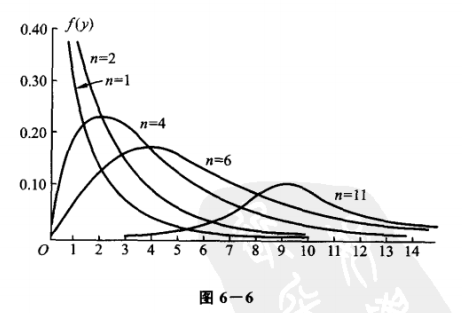
\includegraphics[width=.9\linewidth]{/media/wu/file/stuuudy/notes/images/miscellaneous/6.6.png}
\end{center}
由 \ref{example2.5.3} 及 \ref{example3.5.3} 知\(\chi^2(1)\)服从\(\Gamma(0.5,2)\)分布。现
\(X_i\sim N(0,1)\)由定义\(X_i^2\sim\chi^2(1)\),即\(X_i^2\sim\Gamma(0.5,2)\),
因此
\begin{equation*}
\chi^2=\sum_{i=1}^nX_i^2\sim\Gamma(\frac{n}{2},2)
\end{equation*}

\textbf{\(\chi^2\)分布的可加性} 设\(\chi_1^2\sim\chi^2(n_1),\chi_2^2\sim\chi^2(n_2)\)
 且 \(\chi_1^2,\chi_2^2\)相互独立,则有
\begin{equation*}
\chi_1^2+\chi_2^2\sim\chi^2(n_1+n_2)
\end{equation*}
\textbf{\(\chi^2\)分布的数学期望和方差} 若\(\chi^2\sim\chi^2(n)\),则有
\begin{equation*}
E(\chi^2)=n,D(\chi_2)=2n
\end{equation*}
\textbf{\(\chi^2\)分布的分位点} 对于给定的正数 \(\alpha\) ,\(0<\alpha<1\)称满足条件
\begin{equation*}
P\{\chi^2>\chi_\alpha^2(n)\}=\int_{\chi_\alpha^n}^\infty f(y)dy=\alpha
\end{equation*}
的点\(\chi_\alpha^n(n)\)为\(\chi^2(n)\)分布的上 \(\alpha\) 分位点

\subsubsection{\(t\)分布}
\label{sec:org543e103}
设\(X\sim N(0,1),Y\sim\chi^2(n)\),且\(X,Y\)相互独立,则称随机变量
\begin{equation*}
t=\frac{X}{\sqrt{Y/n}}
\end{equation*}
服从自由度为\(n\)的 \textbf{\(t\)分布} ,记为\(t\sim t(n)\)

\(t\)分布又称 \textbf{学生式(Student)分布} ,\(t(n)\)分布的概率密度函数为
\begin{equation*}
h(t)=\frac{\Gamma((n+1)/2)}{\sqrt{\pi n}\Gamma(n/2)}(1+\frac{t^2}{n})^{-(n+1)/2},
-\infty<t<\infty
\end{equation*}
\begin{equation*}
\lim_{n\to\infty}h(t)=\frac{1}{\sqrt{2\pi}}e^{-t^2/2}
\end{equation*}

\subsubsection{\(F\)分布}
\label{sec:org0eb1d31}
设\(U\sim\chi^2(n_1),V\sim\chi^2(n_2)\),且\(U,V\)相互独立,则称随机变量
\begin{equation*}
F=\frac{U/n_1}{V/n_2}
\end{equation*}
服从自由度\((n_1,n_2)\)的 \textbf{\(F\)分布} ,记为\(F\sim F(n_1,n_2)\)

由定义得
\begin{equation*}
\frac{1}{F}\sim F(n_2,n_1)
\end{equation*}


\(F\)分布的上 \(\alpha\) 分位点有如下性质
\begin{equation*}
F_{1-\alpha}(n_1,n_2)=\frac{1}{F_\alpha(n_2,n_1)}
\end{equation*}

\subsection{正态总体的样本均值与样本方差的分布}
\label{sec:org647007a}
设总体\(X\)的均值为 \(\mu\) ,方差为 \(\sigma^2\),\(X_1,\dots,X_n\)是来自\(X\)的一个样本,
\(\bbar{X},S^2\)分别是样本均值和样本方差,则
\begin{equation*}
E(\bbar{X})=\mu,\quad D(\bbar{X})=\sigma^2/n
\end{equation*}
而
\begin{align*}
E(S^2)&=E\left[\frac{1}{n-1}(\sum_{i=1}^nX_i^2-n\bbar{X}^2)
\right]=\frac{1}{n-1}\left[\sum_{i=1}^nE(X_i^2)-nE(\bbar{X}^2)
\right]\\
&=\frac{1}{n-1}\left[\sum_{i=1}^n(\sigma^2+\mu^2)-n(\sigma^2/n+\mu^2)
\right]=\sigma^2
\end{align*}
即
\begin{equation*}
E(S^2)=\sigma^2
\end{equation*}
进而,设\(X\sim N(\mu,\sigma^2)\),则\(\bbar{X}\)也服从正态分布,则
\begin{theorem}[]
\label{thm6.3.3}
设\(X_1,\dots,X_n\)是来自正态总体\(N(\mu,\sigma^2)\)的样本,\(\bbar{X}\)是样本均值,
则有
\begin{enumerate}
\item \(\bbar{X}\sim N(\mu,\sigma^2/n)\)
\item \(\frac{(n-1)S^2}{\sigma^2}\sim\chi^2(n-1)\)
\item \(\bbar{X}\)与\(S^2\)相互独立
\item \(\frac{\bbar{X}}{S/\sqrt{n}}\sim t(n-1)\)
\end{enumerate}
\end{theorem}

\begin{proof}
\begin{enumerate}
\setcounter{enumi}{1}
\item 设\(Z_i=\frac{X_i-\mu}{\sigma}\),则\(Z_1,\dots,Z_n\)相互独立,而
\begin{gather*}
\bbar{Z}=\frac{1}{n}\sum_{i=1}^nZ_i=\frac{\bbar{X}-\mu}{\sigma}\\
\frac{(n-1)S^2}{\sigma^2}=\frac{\sum_{i=1}^n(X_i-\bbar{X})^2}{\sigma^2}=
\sum_{i=1}^n\left[
\frac{(X_i-\mu)-(\bbar{X}-\mu)}{\sigma}\right]^2\\
=\sum_{i=1}^n(Z_i-\bbar{Z})^2=\sum_{i=1}^nZ_i^2-n\bbar{Z}^2
\end{gather*}
取一\(n\)阶正交矩阵\(\bA=(a_{ij})\),其中第一行的元素均为\(1/\sqrt{n}\),
作正交变换
\begin{equation*}
\bY=\bA\bZ
\end{equation*}
其中
\begin{equation*}
\bY=
\begin{bmatrix}
Y_1\\\vdots\\Y_n
\end{bmatrix},\bZ=
\begin{bmatrix}
Z_1\\\vdots\\Z_n
\end{bmatrix}
\end{equation*}
由于\(Y_i=\displaystyle\sum_{j=1}^na_{ij}Z_j\),故\(Y_1,\dots,Y_n\)仍为正
交变量,由\(Z_i\sim N(0,1)\)知
\begin{equation*}
E(Y_i)=E(\sum_{j=1}^na_{ij}Z_j)=0
\end{equation*}
又由\(Cov(Z_i,Z_j)=\delta_{ij}\),知
\begin{align*}
Cov(Y_i,Y_k)&=Cov(\sum_{j=1}^na_{ij}Z_j,\sum_{l=1}^1a_{kl}Z_l)\\
&=\sum_{j=1}^n\sum_{l=1}^na_{ija_{kl}}Cov(Z_j,Z_l)=\sum_{j=1}^na_{ij}a_{kj}=\delta_{jk}
\end{align*}
故\(Y_1,dots,Y_n\)两两不相关,又由\(n\)维随机变量\((Y_1,\dots,Y_n)\)是由
\(n\)维正态随机变量\((X_1,\dots,X_n)\)经由线性变换得到的,因此
\((Y_1,\dots,Y_n)\)也是\(n\)维正态随机变量,因此\(Y_1,\dots,Y_n\)相互独立,
且有\(Y_i\sim N(0,1)\),而
\begin{gather*}
Y_1=\sum_{j=1}^na_{1j}Z_j=\sum_{j=1}^n\frac{1}{\sqrt{n}}Z_j=\sqrt{n}\bbar{Z}\\
\sum_{i=1}^nY_i^2=\bY^T\bY=(\bA\bZ)^T(\bA\bZ)=\bZ(\bA^T\bA)\bZ=
\bZ^T\bE\bZ=\bZ^T\bZ=\sum_{i=1}^nZ_i^2
\end{gather*}
于是
\begin{equation*}
\frac{(n-1)S^2}{\sigma^2}=\sum_{i=1}^nZ_i^2-n\bbar{Z}^2=\sum_{i=1}^nY_i^2-y_1^2=
\sum_{i=2}^nY_i^2
\end{equation*}

\item \(\bbar{X}=\sigma\bbar{Z}+\mu=\frac{\sigma Y_1}{\sqrt{n}}+\mu\)仅依赖于\(Y_1\)
\item 由 1,2,3
\begin{equation*}
\frac{\bbar{X}-\mu}{\sigma/\sqrt{n}}\sim N(0,1),\quad
\frac{(n-1)S^2}{\sigma^2}\sim\chi^2(n-1)
\end{equation*}
且两者独立,由\(t\)分布的定义知
\begin{equation*}
\left.\frac{\bbar{X}-\mu}{\sigma/\sqrt{n}}\middle/\sqrt{\frac{(n-1)S^2}{\sigma^2(n-1)}}\right.
\sim t(n-1)
\end{equation*}
\end{enumerate}
\end{proof}

\begin{theorem}[]
\label{thm6.3.4}
设\(X_1,\dots,X_{n_1},Y_1,\dots,Y_{n_2}\)分别是来自正态总体\(N(\mu_1,\sigma^2_1)\)
和\(N(\mu_2,\sigma_2^2)\)的样本,且这两个样本相互独立,设
\(\bbar{X}=\frac{1}{n_1}\sum_{i=1}^{n_1}X_i,
   \bbar{Y}=\frac{1}{n_2}\sum_{i=1}^{n_2}Y_i\)为别是两样本的均值,
\(S_1^2,S_2^2\)分别是两样本的样本方差,则有
\begin{enumerate}
\item \(\frac{S_1^2/S_2^2}{\sigma_1^2/\sigma_2^2}\sim F(n_1-1,n_2-1)\)
\item 当\(\sigma_1^2=\sigma_2^2=\sigma^2\)时
\begin{equation*}
\frac{(\bbar{X}-\bbar{Y})-(\mu_1-\mu_2)}{S_w\sqrt{\frac{1}{n_1}+\frac{1}{n_2}}}\sim
t(n_1+n_2-2)
\end{equation*}
其中 \(S_w^2=\frac{(n_1-1)S_1^2+(n_2-1)S_2^2}{n_1+n_2-2},S_w=\sqrt{S_w^2}\)
\end{enumerate}
\end{theorem}

\begin{proof}
\begin{enumerate}
\item \(\hspace{1cm}\)
\begin{equation*}
\frac{(n_1-1)S_1^2}{\sigma_1^2}\sim\chi^2(n_1-1),\frac{(n_2-1)S_2^2}{\sigma_2^2}\sim
\chi^2(n_2-1)
\end{equation*}
由假设\(S_1,S_2\)相互独立,因此
\begin{equation*}
\left.\frac{(n_1-1)S_1^2}{(n_1-1)\sigma_1^1}\middle/
\frac{(n_2-1)S_2^2}{(n_2-1)\sigma_2^2}\right.
\sim F(n_1-1,n_2-1)
\end{equation*}
即
\begin{equation*}
\frac{S_1^2/S_2^2}{\sigma_1^2/\sigma_2^2}\sim F(n_1-1,n_2-1)
\end{equation*}
\item 易知\(\bbar{X}-\bbar{Y}\sim
      N\left(\mu_1-\mu_2,\frac{\sigma^2}{n_1}+\frac{\sigma^2}{n_2}\right)\),即有
\begin{equation*}
U=\frac{(\bbar{X}-\bbar{Y})-(\mu_1-\mu_2)}{
\sigma\sqrt{\frac{1}{n_1}+\frac{1}{n_2}}}\sim N(0,1)
\end{equation*}
又因为
\begin{equation*}
\frac{(n_1-1)S_1^2}{\sigma^2}\sim\chi^2(n_1-1),\frac{(n_2-1)S^2_2}{\sigma^2}
\sim\chi^2(n_2-1)
\end{equation*}
且它们相互独立,故由\(\chi^2\)分布的可加性知
\begin{equation*}
V=\frac{(n_1-1)S_1^2}{\sigma^2}+\frac{(n_2-1)S_2^2}{\sigma^2}\sim\chi^2(n_1+n_2-2)
\end{equation*}
\(U,V\)独立
\end{enumerate}
\end{proof}

\section{参数估计}
\label{sec:orgd3e15a4}
\subsection{点估计}
\label{sec:orgfe1c6f7}
\subsubsection{矩估计法}
\label{sec:orgb1f0ba3}
设\(X\)为连续型随机变量,其概率密度函数为\(f(x;\theta_1,\dots,\theta_k)\),
或\(X\)为离散型随机变量,其分布律为\(P\{X=x\}=p(x;\theta_1,\dots,\theta_k)\),
其中\(\theta_1,\dots,\theta_k\)为待估计参数,\(X_1,\dots,X_n\)是来自\(X\)的
样本,假设总体\(X\)的前\(k\)阶矩
\begin{align*}
 \mu_l&=E(X^l)=\int_{-\infty}^\infty x^lf(x;\theta_1,\dots,\theta_k)dx \quad\text{or}\\
 \mu_l&=E(X^l)=\sum_{x\in R_X}x^lp(x;\theta_1,\dots,\theta_k)
\end{align*}
其中\(R_X\)是\(X\)的取值范围,基于样本矩
\begin{equation*}
A_l=\frac{1}{n}\sum_{i=1}^nX_i^l
\end{equation*}
依概率收敛于相应的总体矩\(\mu_l\),样本矩的连续函数依概率收敛于相应的总体矩的
连续函数,我们就用样本矩作为相应的总体矩的估计量,而以样本矩的连续函数作为相
应的总体矩的连续函数的估计量,这种估计方法称为 \textbf{矩估计法} 。具体做法如下,设
\begin{equation*}
\begin{cases}
\mu_1=\mu_1(\theta_1,\dots,\theta_k)\\
\mu_2=\mu_2(\theta_1,\dots,\theta_k)\\
\vdots\\
\mu_k=\mu_k(\theta_1,\dots,\theta_k)\\
\end{cases}
\end{equation*}
这是一个包含\(k\)个未知参数\(\theta_1,\dots,\theta_k\)的联立方程组,可解出
\begin{equation*}
\begin{cases}
\theta_1=\theta_1(\mu_1,\dots,\mu_k)\\
\theta_2=\theta_2(\mu_1,\dots,\mu_k)\\
\vdots\\
\theta_k=\theta_k(\mu_1,\dots,\mu_k)\\
\end{cases}
\end{equation*}
以\(A_i\)分别代替上式中的 \(\mu_i\),就以
\begin{equation*}
\hat{\theta}_i=\theta_i(A_1,\dots,A_k)
\end{equation*}
分别作为\(\theta_i\)的估计量,这种估计量称为 \textbf{矩估计量} ,矩估计量的观察值称为
\textbf{矩估计值}

\begin{examplle}[]
设总体\(X\)在\([a,b]\)上服从均匀分布,\(a,b\)未知,\(X_1,\dots,X_n\)是来自
\(X\)的样本,试求\(a,b\)的矩估计量

\begin{align*}
\mu_1&=E(X)=(a+b)/2\\
\mu_2&=E(X^2)=D(X)+[E(X)]^2=(b-a)^2/12+(a+b)^2/4
\end{align*}
解得
\begin{equation*}
a=\mu_1-\sqrt{3(\mu_2-\mu_1^2)},b=\mu_1+\sqrt{3(\mu_2-\mu_1^2)}
\end{equation*}
e 分别以\(A_1,A_2\)代替\(\mu_1,\mu_2\)
\end{examplle}

\begin{examplle}[]
设总体\(X\)的均值 \(\mu\) 及方差 \(\sigma^2\)都存在,且有\(\sigma^2>0\),但\(\mu,\sigma^2\)均未知,
又设\(X_1,\dots,X_n\)是来自\(X\)的样本,试求\(\mu,\sigma^2\)的矩估计量

\begin{equation*}
\begin{cases}
\mu_1=E(X)=\mu\\
\mu_2=E(X^2)=\sigma^2+\mu^2
\end{cases}
\end{equation*}
解得
\begin{equation*}
\begin{cases}
\mu=\mu_1\\
\sigma^2=\mu_2-\mu_1^2
\end{cases}
\end{equation*}
因此
\begin{align*}
\hat{\mu}&=A_1=\bbar{X}\\
\hat{\sigma}^2&=A_2-A_1^2=\frac{1}{n}\sum_{i=1}^nX_i^2-\bbar{X}^2=
\frac{1}{n}\sum_{i=1}^n(X_i-\bbar{X})^2
\end{align*}
\end{examplle}
\subsubsection{最大似然估计法}
\label{sec:org29e8ad7}
若总体\(X\)属于离散型,其分布律\(P\{X=x\}=p(x;\theta),\theta\in\Theta\)的形式已知,
\(\theta\)为待沽参数, \(\Theta\) 是 \(\theta\) 可能取值的范围,设\(X_1,\dots,X_n\)是来自\(X\)
的样本,则\(X_1,\dots,X_n\)的联合分布
\begin{equation*}
\prod_{i=1}^np(x_1;\theta)
\end{equation*}
又设\(x_1,\dots,x_n\)是相应于\(X_1,\dots,X_n\)的样本值,则事件
\(\{X_1=x_1,\dots,X_n=x_n\}\)发生的概率为
\begin{equation*}
L(\theta)=L(x_1,\dots,x_n;\theta)=\prod_{i=1}^np(x_i;\theta),\theta\in\Theta
\end{equation*}
\(L(\theta)\)称为样本的 \textbf{似然函数} 。取\(\hat{\theta}\)使
\begin{equation*}
L(x_1,\dots,x_n;\hat{\theta})=\max_{\theta\in\Theta}L(x_1,\dots,x_n;\theta)
\end{equation*}
这样得到的\(\hat{\theta}\)与样本值\(x_1,\dots,x_n\)有关,常记为
\(\hat{\theta}(x_1,\dots,x_n)\),称为参数 \(\theta\) 的 \textbf{最大似然估计值} ,而相应的统计量
\(\hat{\theta}(X_1,\dots,X_n)\)称为参数 \(\theta\) 的 \textbf{最大似然估计量}

若总体\(X\)属连续型,其概率密度\(f(x;\theta),\theta\in\Theta\)的形式已知,设
\(X_1,\dots,X_n\)是来自\(X\)的样本,它们的联合密度为
\begin{equation*}
\prod_{i=1}^nf(x_i,\theta)
\end{equation*}
设\(x_1,\dots,x_n\)是相应于样本\(X_1,\dots,X_n\)的一个样本值,则随机点
\((X_1,\dots,X_n)\)落在点\((x_1,\dots,x_n)\)的邻域(变长分别为
\(dx_1,\dots,dx_n\)的\(n\)维立方体)内的概率近似地为
\begin{equation*}
\prod_{i=1}^nf(x_i;\theta)dx_i
\end{equation*}
因因子\(\prod_{i=1}^ndx_i\)不随 \(\theta\) 改变,故只需考虑函数
\begin{equation*}
L(\theta)=L(x_1,\dots,x_n;\theta)=\prod_{i=1}^nf(x_i;\theta)
\end{equation*}
的最大值,这里\(L(\theta)\)称为样本的 \textbf{似然函数} ,若
\begin{equation*}
L(x_1,\dots,x_n;\hat{\theta})=\max_{\theta\in\Theta}L(x_1,\dots,x_n;\theta)
\end{equation*}
则称\(\hat{\theta}(x_1,\dots,x_n)\)为 \(\theta\) 的 \textbf{最大似然估计值} ,称
\(\hat{\theta}(X_1,\dots,X_n)\)为 \(\theta\) 的 \textbf{最大似然估计量}

很多时候\(p(x;\theta),f(x;\theta)\)关于 \(\theta\) 可微,因此 \(\theta\) 的最大似然估计可以从方程
\begin{equation*}
\frac{d}{d\theta}\ln L(\theta)=0
\end{equation*}
求得, 这个方程称为 \textbf{对数似然方程}

\begin{examplle}[]
设\(X\sim(1,p)\),\(X_1,\dots,X_n\)是来自\(X\)的一个样本,求参数\(p\)的最大 r
似然估计

设\(x_1,\dots,x_n\)是相应于样本\(X_1,\dots,X_n\)的一个样本值,\(X\)的分布律
为
\begin{equation*}
P\{X=x\}=p^2(1-p)^{1-x},x=0,1
\end{equation*}
故
\begin{gather*}
L(p)=\prod_{i=1}^np^{x_i}(1-p)^{1-x_i}=p^{\sum_{i=1}^nx_i}(1-p)^{n-\sum_{i=1}^nx_i}\\
\ln L(p)=(\sum_{i=1}^nx_i)\ln p+(n-\sum_{i=1}^nx_i)\ln(1-p)\\
\frac{d}{dp}\ln L(p)=\frac{\sum_{i=1}^nx_i}{p}-\frac{n-\sum_{i=1}^nx_i}{1-p}=0\\
\hat{p}=\frac{1}{n}\sum_{i=1}^nx_i=\bbar{x}
\end{gather*}
\end{examplle}

\begin{examplle}[]
设\(X\sim N(\mu,\sigma^2)\), \(\mu\),\(\sigma\) 未知,\(x_1,\dots,x_n\)是来自\(X\)的一个样本值,
求\(\mu,\sigma^2\)的最大似然估计函数

\(X\)的概率密度函数
\begin{equation*}
f(x;\mu,\sigma^2)=\frac{1}{\sqrt{2\pi}\sigma}\exp\left[
-\frac{1}{2\sigma^2}(x-\mu^2)
\right]
\end{equation*}
似然函数为
\begin{align*}
L(\mu,\sigma^2)&=\prod_{i=1}^n\frac{1}{\sqrt{2\pi}\sigma}\exp\left[
-\frac{1}{2\sigma^2}(x-\mu^2)
\right]\\
&=(2\pi)^{-n/2}(\sigma^2)^{-n/2}\exp\left[
-\frac{1}{2\sigma^2}\sum_{i=1}^n(x_i-\mu)^2
\right]\\
\ln L&=-\frac{n}{2}\ln(2\pi)-\frac{n}{2}\ln\sigma^2-\frac{1}{2\sigma^2}\sum_{i=1}^n(x_i-\mu)^2
\end{align*}
令
\begin{equation*}
\begin{cases}
\frac{\partial}{\partial \mu}\ln L=\frac{1}{\sigma^2}(\sum_{i=1}^nx_i-n\mu)=0\\
\frac{\partial}{\partial\sigma^2}\ln L=
-\frac{n}{2\sigma^2}+\frac{1}{2(\sigma^2)^2}\sum_{i=1}^n(x_i-\mu)^2=0
\end{cases}
\end{equation*}
解得
\begin{equation*}
\hat{\mu}=\bbar{X},\quad\hat{\sigma}^2=\frac{1}{n}\sum_{i=1}^n(X_i-\bbar{X})^2
\end{equation*}
\end{examplle}

\begin{examplle}[]
设总体\(X\)在\([a,b]\)上服从均匀分布,\(a,b\)未知,\(x_1,\dots,x_n\)是一个样
本值,求\(a,b\)的最大似然估计函数
记\(x_{(1)}=\min\{x_1,\dots,x_n\},x_{(n)}=\max\{x_1,\dots,x_n\}\),\(X\)的概
率密度是
\begin{equation*}
f(x;a,b)=
\begin{cases}
\frac{1}{b-a}&a\le x\le b\\
0&
\end{cases}
\end{equation*}
似然函数为
\begin{equation*}
L(a,b)=
\begin{cases}
\frac{1}{(b-a)^n}&a\le x_1,\dots,x_n\le b\\
0&
\end{cases}
\end{equation*}
由于\(a\le x_1,\dots,x_n\le b\)等价于\(a\le x_{(1)},x_{(n)}\le b\)似然函数可
写成
\begin{equation*}
L(a,b)=
\begin{cases}
\frac{1}{(b-a)^n}&a\le x_{(1)},b\ge x_{(n)}\\
0&
\end{cases}
\end{equation*}
于是对于满足条件\(a\le x_{(1)},b\ge x_{(n)}\)的任意\(a,b\)有
\begin{equation*}
L(a,b)=\frac{1}{(b-a)^n}\le\frac{1}{(x_{(n)}-x_{(1)})^n}
\end{equation*}
即\(L(a,b)\)在\(a=x_{(1)},b=x_{(n)}\)时取得最大值,故\(a,b\)的最大似然估计值
为
\begin{equation*}
\hat{a}=x_{(1)},\hat{b}=x_{(n)}
\end{equation*}
\end{examplle}

此外,最大似然估计具有下述性质:设 \(\theta\) 的函数\(u=u(\theta),\theta\in\Theta\)具有单
值反函数\(\theta=\theta(u),u\in\calu\),又假设\(\hat{\theta}\)是\(X\)的概率分布中
参数 \(\theta\) 的最大似然估计,则\(\hat{u}=u(\hat{\theta})\)是\(u(\theta)\)的最大似然估计,这
一性质称为最大似然估计的 \textbf{不变性}
\subsection{基于截尾样本的最大似然估计}
\label{sec:org3f39bad}
将随机抽取的\(n\)个产品在\(t=0\)时投入试验直到每个产品都失效,记录每一个产品
的 失效时间,这样的道德样本叫完全样本。 截尾寿命试验有两种:定时截尾寿命试验,
假设将随机抽取的\(n\)个产品在\(t=0\)投入试验,试验进行到事先规定的截尾时间
\(t_0\)停止,如试验截止时共有\(m\)个产品失效,它们的失效时间分别为
\begin{equation*}
0\le t_1\le \dots\le t_m\le t_0
\end{equation*}
此时\(m\)是一个随机变量,所得的样本\(t_1,\dots,t_m\)称为 \textbf{定时截尾样本} 。另一
种是定数截尾样本, \(t_m\)是第\(m\)个产品的失效时间,所得到的样本
\(t_1\dots t_m\)称为 \textbf{定数截尾样本}

设产品的寿命分布为指数分布
\begin{equation*}
f(t)=
\begin{cases}
\frac{1}{\theta}e^{-t/\theta}&t>0\\
0&
\end{cases}
\end{equation*}
设有\(n\)个产品投入定数截尾试验。
一个产品在\((t_i,t_i+dt_i]\)失效的概率近似地为
\(f(t_i)dt_i=\frac{1}{\theta}e^{-t_i/\theta}dt_i\),其余\(n-m\)个产品寿命超过
\(t_m\)的概率为
\((\int_{t_m}^\infty\frac{1}{\theta}e^{-t/\theta}dt)^{n-m}=(e^{-t_m/\theta})^{n-m}\)
,故上述观察结果出现的概率近似地为
\begin{align*}
&\binom{n}{m}(\frac{1}{\theta}e^{-t_1/\theta}t_1)\dots(\frac{1}{\theta}e^{-t_m/\theta}t_m)
(e^{-t_m/\theta})^{n-m}\\
&\quad=\binom{n}{m}\frac{1}{\theta^m}e^{-\frac{1}{\theta}[t_1+\dots+t_m+(n-m)t_m]}dt_1\dots dt_m
\end{align*}
其中\(dt_1,\dots,dt_m\)为常数,因忽略常数不影响 \(\theta\) 的最大似然估计,
故可取似然函数为
\begin{equation*}
L(\theta)=\frac{1}{\theta^m}e^{-\frac{1}{\theta}[t_1+\dots+t_m+(n-m)t_m]}
\end{equation*}
则
\begin{equation*}
\frac{d}{d\theta}\ln L(\theta)=-\frac{m}{\theta}+\frac{1}{\theta^2}[t_1+\dots+t_m+(n-m)t_m]=0
\end{equation*}
于是
\begin{equation*}
\hat{\theta}=\frac{s(t_m)}{m}
\end{equation*}
其中\(s(t_m)=t_1+\dots+t_m+(n-m)t_m\)称为总试验时间

对于截尾样本
\begin{equation*}
0\le t_1\le \dots\le t_m\le t_0
\end{equation*}
可得
\begin{gather*}
L(\theta)=\frac{1}{\theta^m}e^{-\frac{1}{\theta}[t_1+\dots+t_m+(n-m)t_0]}\\
\hat{\theta}=\frac{s(t_0)}{m}
\end{gather*}
其中\(s(t_0)=t_1+\dots+t_m+(n-m)t_0\)
\subsection{评估量的评选标准}
\label{sec:orge89c783}
\subsubsection{无偏性}
\label{sec:org5763b92}
设\(X_1,\dots,X_n\)是总体\(X\)的一个样本,\(\theta\in\Theta\)是包含在总体
\(X\)的分布中的待沽参数,这里 \(\Theta\) 是 \(\theta\) 的取值范围

\begin{definition}[]
若估计量\(\hat{\theta}=\hat{\theta}(X_1,\dots,X_n)\)的数学期望\(E(\hat{\theta})\)存在,且对
于任意\(\theta\in\Theta\)有
\begin{equation*}
E(\hat{\theta})=\theta
\end{equation*}
则称\(\hat{\theta}\)是 \(\theta\) 的 \textbf{无偏估计量}
\end{definition}

\begin{examplle}[]
设总体\(X\)的\(k\)阶矩\(\mu_k=E(X^k)\)存在,又设\(X_1,\dots,X_n\)是\(X\)的一
个样本,试证明不论总体服从什么分布,\(k\)阶样本矩
\(A_k=\frac{1}{n}\sum_{i=1}^nX_i^k\)是\(k\)阶总体矩\(\mu_k\)的无偏估计

\(X_1,\dots,X_n\)与\(X\)同分布,故有
\begin{equation*}
E(X_i^k)=E(X^k)=\mu_k
\end{equation*}
\end{examplle}

\begin{examplle}[]
设总体\(X\)服从指数分布,其概率密度为
\begin{equation*}
f(x;\theta)=
\begin{cases}
\frac{1}{\theta}e^{-x/\theta}&x>0\\0
\end{cases}
\end{equation*}
其中\(\theta>0\)未知,又设\(X_1,\dots,X_n\)是来自\(X\)的样本,证明
\(nZ=n(\min\{X_1,\dots,X_n\})\)是\(\theta\)的无偏估计

\(Z=\min\{X_1,\dots,X_n\}\)具有概率密度
\begin{equation*}
f_{\min}(x;\theta)=
\begin{cases}
\frac{n}{\theta}e^{-nx/\theta}&x>0\\0
\end{cases}
\end{equation*}
故
\begin{equation*}
E(Z)=\frac{\theta}{n}
\end{equation*}
\end{examplle}
\subsubsection{有效性}
\label{sec:orgd884199}
\begin{definition}[]
设\(\hat{\theta}_1=\hat{\theta}_1(X_1,\dots,X_n),\hat{\theta}_2=\hat{\theta}_2(X_1,\dots,X_n)\)
都是 \(\theta\) 的无偏估计量,若对于任意\(\theta\in\Theta\)
\begin{equation*}
D(\hat{\theta}_1)\le D(\hat{\theta}_2)
\end{equation*}
且至少对于某一个\(\theta\in\Theta\)上式不等号成立,则称\(\hat{\theta}_1\)比
\(\hat{\theta}_2\) \textbf{有效}
\end{definition}
\subsubsection{相合性}
\label{sec:org98d06a4}
\begin{definition}[]
设\(\hat{\theta}(X_1,\dots,X_n)\)为参数 \(\theta\) 的估计量,若对于任意\(\theta\in\Theta\),
当\(n\to\infty\)时\(\hat{\theta}(X_1,\dots,X_n)\)依概率收敛于 \(\theta\) ,则称\(\hat{\theta}\)
为 \(\theta\) 的 \textbf{相合估计量}
\end{definition}
\subsection{区间估计}
\label{sec:org208a244}
\begin{definition}[]
设总体\(X\)的分布函数\(F(x;\theta)\)含有一个未知数\(\theta\in\Theta\),对于给定值
\(\alpha(0<\alpha<1)\)若由来自\(X\)的样本\(X_1,\dots,X_n\)确定的两个统计量
\(\und{\theta}<\bbar{\theta}\)对于任意\(\theta\in\Theta\)满足
\begin{equation*}
P\{\und{\theta}(X_1,\dots,X_n)<\theta<\bbar{\theta}(X_1,\dots,X_n)\}\ge1-\alpha
\end{equation*}
则称随机区间 \((\und{\theta},\bbar{\theta})\)是 \(\theta\) 的置信水平为 \(1-\alpha\) 的 \textbf{置信区
间} ,\(\und{\theta},\bbar{\theta}\)分别是双侧置信区间的 \textbf{置信下限} 和 \textbf{置信下限} ,
\(1-\alpha\)为 \textbf{置信水平}
\end{definition}

\begin{examplle}[]
设总体\(X\sim N(\mu,\sigma^2)\),\(\sigma^2\)已知, \(\mu\) 未知,设\(X_1,\dots,X_n\)是来自
\(X\)的样本,求 \(\mu\) 的置信水平为 \(1-\alpha\)的置信区间

\(\bbar{X}\)是 \(\mu\) 的无偏估计,且有
\begin{equation*}
\frac{\bbar{X}-\mu}{\sigma/\sqrt{n}}\sim N(0,1)
\end{equation*}
因此按正态分布
\begin{equation*}
P\{\abs{\frac{\bbar{X}-\mu}{\sigma/\sqrt{n}}}<z_{\alpha/2}\}=1-\alpha
\end{equation*}
即
\begin{equation*}
P\{\bbar{X}-\frac{\sigma}{\sqrt{n}}z_{\alpha/2}<\mu<\bbar{X}+\frac{\sigma}{\sqrt{n}}z_{\alpha/2}\}=1-\alpha
\end{equation*}
因此得到了 \(\mu\) 的一个置信水平为 \(1-\alpha\)的置信区间
\begin{equation*}
\left(\bbar{X}-\frac{\sigma}{\sqrt{n}}z_{\alpha/2},\bbar{X}+\frac{\sigma}{\sqrt{n}}z_{\alpha/2}\right)
\end{equation*}
\end{examplle}

寻求未知参数 \(\theta\) 的置信区间的做法
\begin{enumerate}
\item 寻求一个样本\(X_1,\dots,X_n\)和 \(\theta\) 的函数\(W=W(X_1,\dots,X_n;\theta)\)使得\(W\)
的分布不依赖于 \(\theta\) 以及其他未知参数,称具有这种性质的函数\(W\)为 \textbf{枢轴量}
\item 对于给定的置信水平 \(1-\alpha\)定出两个常数\(a,b\),使得
\begin{equation*}
P\{a<W(X_1,\dots,X_n;\theta)<b\}=1-\alpha
\end{equation*}
\end{enumerate}

\subsection{正态总体均值与方差的区间估计}
\label{sec:org84763fd}
\subsubsection{单个总体\(N(μ,σ^2)\)的情况}
\label{sec:org094e3ee}
设已给定置信水平为\(1-\alpha\),并设\(X_1,\dots,X_n\)为总体\(N(\mu,\sigma^2)\)的样
本,\(\bbar{X},S^2\)分别是样本均值和样本方差
\begin{enumerate}
\item 均值 \(\mu\) 的置信区间
\begin{enumerate}
\item \(\sigma^2\)为已知,得到
\begin{equation*}
\left(\bbar{X}\pm\frac{\sigma}{\sqrt{n}}z_{\alpha/2}
\right)
\end{equation*}
\item \(\sigma^2\)未知,考虑\(S^2\)是\(\sigma^2\)的无偏估计,由定理 \ref{thm6.3.3}
\begin{equation*}
\frac{\bbar{X}-\mu}{S/\sqrt{n}}\sim t(n-1)
\end{equation*}
因此得 \(\mu\) 的一个置信水平为\(1-\alpha\)的置信区间
\begin{equation*}
\left(\bbar{X}\pm\frac{S}{\sqrt{n}}t_{\alpha/2}(n-1)
\right)
\end{equation*}
\end{enumerate}
\item 方差\(\sigma^2\)的置信区间
\(\mu\) 未知,\(\sigma^2\)的无偏估计为\(S^2\)
\begin{equation*}
\frac{(n-1)S^2}{\sigma^2}\sim\chi^2(n-1)
\end{equation*}
有
\begin{equation*}
P\left\{\chi_{1-\alpha/2}^2(n-1)<\frac{(n-1)S^2}{\sigma^2}<\chi_{\alpha/2}^2(n-1)
\right\}=1-\alpha
\end{equation*}
因此得到方差\(\sigma^2\)的一个置信水平为\(1-\alpha\)的置信区间
\begin{equation*}
\left(\frac{(n-1)S^2}{\chi_{\alpha/2}^2(n-1)},\frac{(n-1)S^2}{\chi_{1-\alpha/2}^2(n-1)}
\right)
\end{equation*}
\end{enumerate}
\subsubsection{两个总体\(N(μ_1,σ^2_1),N(μ_2,σ^2_2)\)的情况}
\label{sec:org501e14c}
设给定置信水平\(1-\alpha\),并设\(X_1,\dots,X_{n_1}\)是来自第一个总体的样本;
\(Y_1,\dots,Y_{n_2}\)是来自第二个总体的样本,这两个样本相互独立,且设
\(\bbar{X},\bbar{Y},S_1^2,S_2^2\)分别是第一、二个总体的样本均值、方差
\begin{enumerate}
\item 两个总体均值差\(\mu_1-\mu_2\)的置信区间
\begin{enumerate}
\item \(\sigma_1^2,\sigma_2^2\)均为已知,则
\begin{equation*}
\bbar{X}-\bbar{Y}\sim N(\mu_1-\mu_2,\frac{\sigma_1^2}{n_1}+\frac{\sigma_2^2}{n_2})
\end{equation*}
因此得到\(\mu_1-\mu_2\)的一个置信水平为\(1-\alpha\)的置信区间
\begin{equation*}
\left(\bbar{X}-\bbar{Y}\pm z_{\alpha/2}\sqrt{\frac{\sigma_1^2}{n_1}+\frac{\sigma_2^2}{n_2}}
\right)
\end{equation*}
\item \(\sigma_1^2=\sigma_2^2=\sigma^2\),但\(\sigma^2\)未知,此时由定理
\ref{thm6.3.4}
\begin{equation*}
\frac{(\bbar{X}-\bbar{Y})-(\mu_1-\mu_2)}{S_w\sqrt{\frac{1}{n_1}+\frac{1}{n_2}}}
\sim t(n_1+n_2-2)
\end{equation*}
可得\(\mu_1-\mu_2\)的一个置信水平为\(1-\alpha\)的置信区间为
\begin{equation*}
\left(
\bbar{X}-\bbar{Y}\pm t_{\alpha/2}(n_1+n_2-2)S_w\sqrt{\frac{1}{n_1}+\frac{1}{n_2}}
\right)
\end{equation*}
此处
\begin{equation*}
S_2^2=\frac{(n_1-1)S_1^2+(n_2-1)S_2^2}{n_1+n_2-2},S_w=\sqrt{S_w^2}
\end{equation*}
\end{enumerate}
\item 两个总体方差比\(\sigma_1^2/\sigma_2^2\)的置信区间
\(\mu_1,\mu_2\)均未知,由定理 \ref{thm6.3.4}
\begin{equation*}
\frac{S_1^2/S_2^2}{\sigma_1^2/\sigma_2^2}\sim F(n_1-1,n_2-1)
\end{equation*}
有
\begin{equation*}
P\left\{
F_{1-\alpha/2}(n_1-1,n_2-1)<\frac{S_1^2/S_2^2}{\sigma_1^2/\sigma_2^2}<
F_{\alpha/2}(n_1-1,n_2-1)
\right\}=1-\alpha
\end{equation*}
因此得\(\sigma_1^2/\sigma_2^2\)的一个置信水平为\(1-\alpha\)的置信区间
\begin{equation*}
\left(
\frac{S_1^2}{S_2^2}\frac{1}{F_{\alpha/2}(n_1-1,n_2-1)},
\frac{S_1^2}{S_2^2}\frac{1}{F_{1-\alpha/2}(n_1-1,n_2-1)}
\right)
\end{equation*}
\end{enumerate}
\subsection{\((0-1)\)分布参数的区间估计}
\label{sec:orgbbb6996}
设有一容量\(n>50\)的大样本,它来自\((0-1)\)分布的总体\(X\),\(X\)的分布律为
\begin{equation*}
f(x;p)=p^x(1-p)^{1-x},x=0,1
\end{equation*}
其中\(p\)为未知参数,现在求\(p\)的置信水平为\(1-\alpha\)的置信区间

已知\((0-1)\)分布的均值和方差分别为
\begin{equation*}
\mu=p,\sigma^2=p(1-p)
\end{equation*}
设\(X_1,\dots,X_n\)是一个样本,因样本容量\(n\)较大,由中心极限定理,知
\begin{equation*}
\frac{n\bbar{X}-np}{\sqrt{np(1-p)}}\sim N(0,1)
\end{equation*}
于是有
\begin{equation*}
P\left\{
-z_{\alpha/2}<\frac{n\bbar{X}-np}{\sqrt{np(1-p)}}<z_{\alpha/2}
\right\}\approx 1-\alpha
\end{equation*}
而不等式
\begin{equation*}
-z_{\alpha/2}<\frac{n\bbar{X}-np}{\sqrt{np(1-p)}}<z_{\alpha/2}
\end{equation*}
等价于
\begin{equation*}
(n+z_{\alpha/2}^2)p^2-(2n\bbar{X}+z_{\alpha/2}^2)p+n\bbar{X}^2< 0
\end{equation*}
记
\begin{align*}
p_1&=\frac{1}{2a}(-b-\sqrt{b^2-4ac})\\
p_2&=\frac{1}{2a}(-b+\sqrt{b^2-4ac})
\end{align*}
此处\(a=n+z_{\alpha/2}^2,b=-(2n\bbar{X}+z_{\alpha/2}^2),c=n\bbar{X}^2\),于是
得置信区间
\begin{equation*}
(p_1,p_2)
\end{equation*}
\subsection{单侧置信区间}
\label{sec:orgd2acafc}
对于给定值\(\alpha(0<\alpha<1)\)若由样本\(X_1,\dots,X_n\)确定的统计量
\(\und{\theta}=\und{\theta}(X_1,\dots,X_n)\)对于任意\(\theta\in\Theta\)满足
\begin{equation*}
P\{\theta>\und{\theta}\}\ge 1-\alpha
\end{equation*}
称随机区间\((\und{\theta},\infty)\)是 \(\theta\) 的置信水平为 \(1-\alpha\)的 \textbf{单侧置信区间}
,\(\und{\theta}\)称为 \(\theta\) 的置信为凭为 \(1-\alpha\)的单侧置信上限

若对于正态总体\(X\),若均值 \(\mu\) ,方差\(\sigma^2\)均未知,设\(X_1,\dots,X_n\)是一个样
本,由
\begin{equation*}
\frac{\bbar{X}-\mu}{S/\sqrt{n}}\sim t(n-1)
\end{equation*}
有
\begin{equation*}
P\{\frac{\bbar{X}-\mu}{S/\sqrt{n}}<t_\alpha(n-1)\}=1-\alpha
\end{equation*}
因此得到 \(\mu\)  的一个置信水平为 \(1-\alpha\)的单侧置信区间
\begin{equation*}
\left(
\bbar{X}-\frac{S}{\sqrt{n}}t_\alpha(n-1),\infty
\right)
\end{equation*}
\section{假设检验}
\label{sec:orgf2cf069}
\subsection{假设检验}
\label{sec:orgda207f4}

\begin{examplle}[]
某车间用一台包装机包装葡萄糖,袋装糖的净重是一个随机变量,它服从正态分布,当
机器正常时,其均值为 0.5 kg,标准差为 0.015kg,某日开工后为检验包装机是否正常,
随机地抽取它所包装的糖 9 袋,称得净重为(kg)
\begin{center}
\begin{tabular}{rrrrrrrrr}
0.497 & 0.506 & 0.518 & 0.524 & 0.498 & 0.511 & 0.520 & 0.515 & 0.512\\
\end{tabular}
\end{center}
问机器是否正常
\end{examplle}

以 \(\mu\),\(\sigma\) 分别表示这一天袋装糖的净重总体\(X\)的均值和标准差。由于标准差比较稳定,
设\(\sigma=0.015\),
于是\(X\sim N(\mu,0.015^2)\),这里 \(\mu\) 未知,问题是根据样本值来判断 \(\mu\) 是否等于 0.5。
为此我们提出两个相互对立的假设
\begin{align*}
&H_0:\mu=\mu_0=0.5\\
&H_1:\mu\neq\mu_0
\end{align*}

\(\bbar{X}\)是 \(\mu\)  的无偏估计,\(\bbar{X}\)的观察值\(\bbar{x}\)的大小在一定程
度上反映 \(\mu\) 的大小。如果假设\(H_0\)为真,则观察值\(\bbar{x}\)与\(\mu_0\)的偏差
\(\abs{\bbar{x}-\mu_0}\)一般不应太大

\(P_{\mu_0}\{\cdot\}\)表示参数 \(\mu\)  取 \(\mu_0\)时事件的概率,\(P_{\mu\in
   H_0}\{\cdot\}\)表示 \(\mu\) 取\(H_0\)规定的值时事件\(\{\cdot\}\)的概率。我们希望
\begin{equation*}
P\{\text{当$H_0$为真拒绝$H_0$}\}\le\alpha
\end{equation*}
由于只允许犯这类错误的概率最大为 \(\alpha\) ,因此
\begin{equation*}
P_{\mu_0}\left\{
\abs{\bbar{X}-\mu_0}{\sigma/\sqrt{n}}\ge k
\right\}=\alpha
\end{equation*}
由于当\(H_0\)为真时,\(Z=\frac{\bbar{X}-\mu_0}{\sigma/\sqrt{n}}\sim N(0,1)\),
因此
\begin{equation*}
k=a_{\alpha/2}
\end{equation*}
因此若\(Z\)的观察值满足
\begin{equation*}
\abs{z}=\frac{\bbar{x}-\mu_0}{\sigma/\sqrt{n}}\ge k=z_{\alpha/2}
\end{equation*}
则拒绝\(H_0\),反之接受

数 \(\alpha\) 称为 \textbf{显著水平} ,统计量\(Z=\frac{\bbar{X}-\mu_0}{\sigma/\sqrt{n}}\)称为
\textbf{检验统计量}

在显著水平 \(\alpha\) 下,检验假设
\begin{equation*}
H_0:\mu=\mu_0,\quad H_1:\mu\neq\mu_0
\end{equation*}
\(H_0\)称为 \textbf{原假设} 或 \textbf{零假设} ,\(H_1\)称为 \textbf{备择假设}

当检验统计量取某个区域\(C\)中的值时,我们拒绝原假设\(H_0\),则称区域\(C\)为
\textbf{拒绝域} ,拒绝域的边界点称为 \textbf{临界点}

\(H_0\)为真时拒绝称为第\rom{1}类错误,\(H_0\)不真时接收\(H_0\)称为第\rom{2}类
错误

只对犯第\rom{1}类错误的概率加以控制而不考虑第\rom{2}类错误的概率的检验称为 \textbf{显
著性检验} 。

\begin{equation*}
H_0:\mu\le\mu_0,\quad H_1:\mu>\mu_0
\end{equation*}
称为 \textbf{右边检验}
\begin{equation*}
H_0:\mu\ge\mu_0,\quad H_1:\mu<\mu_0
\end{equation*}
称为 \textbf{左边检验} 。左边检验和右边检验统称为 \textbf{单边检验}

设总体\(X\sim N(\mu,\sigma^2)\), \(\mu\) 未知, \(\sigma\) 已知,\(X_1,\dots,X_n\)是来自\(X\)的样
本,给定显著性水平 \(\alpha\) ,求检验问题
\begin{equation*}
H_0:\mu\le \mu_0,\quad H_1:\mu>\mu_0
\end{equation*}
的拒绝域

因\(H_0\)中的全部 \(\mu\) 都比 \(H_1\)中的 \(\mu\) 要小,当\(H_1\)为真时,观察值
\(\bbar{x}\)往往偏大,因此拒绝域的形式为
\begin{equation*}
\bbar{x}\ge k
\end{equation*}
则
\begin{align*}
P_{\mu\in H_0}{\bbar{X}\ge k}&=
P_{\mu\le \mu_0}\left\{
\frac{\bbar{X}-\mu_0}{\sigma/\sqrt{n}}\ge\frac{k-\mu_0}{\sigma/\sqrt{n}}
\right\}\\
&\le P_{\mu\le \mu_0}\left\{
\frac{\bbar{X}-\mu}{\sigma/\sqrt{n}}\ge\frac{k-\mu_0}{\sigma/\sqrt{n}}
\right\}
\end{align*}
要控制\(P\{\text{当$H_0$为真拒绝$H_0$}\}\le\alpha\)只需令
\begin{equation*}
P_{\mu\le \mu_0}\left\{
\frac{\bbar{X}-\mu}{\sigma/\sqrt{n}}\ge\frac{k-\mu_0}{\sigma/\sqrt{n}}
\right\}=\alpha
\end{equation*}
因此
\(\frac{k-\mu_0}{\sigma/\sqrt{n}}=z_\alpha,k=\mu_0+\frac{\sigma}{sqrt{n}z_\alpha}\)
,即得拒绝域为
\begin{equation*}
\bbar{x}\ge\mu_0+\frac{\sigma}{\sqrt{n}}z_\alpha
\end{equation*}

同理得左边检验问题
\begin{equation*}
 H_0:\mu\ge \mu_0,\quad H_1:\mu<\mu_0
\end{equation*}
的拒绝域为
\begin{equation*}
z=\frac{\bbar{x}-\mu_0}{\sigma/\sqrt{n}}\le-z_\alpha
\end{equation*}
\subsection{正态总体均值的假设检验}
\label{sec:orgff8811c}
\subsubsection{单个总体\(N(μ,σ^2)\)均值\(μ\)检验}
\label{sec:org877bf05}
\begin{enumerate}
\item \(\sigma^2\)已知,关于 \(\mu\) 检验(\(Z\)检验)
利用统计量\(Z=\frac{\bbar{X}-\mu_0}{\sigma/\sqrt{n}}\)来确定拒绝域,称为
\textbf{\(Z\)检验法}
\item \(\sigma^2\)未知,关于 \(\mu\) 的检验(\(t\)检验)
设总体\(X\sim N(\mu,\sigma^2)\),其中\(\mu,\sigma^2\)未知,求检验问题
\begin{equation*}
H_0:\mu=\mu_0,\quad H:\mu\neq\mu_0
\end{equation*}
的拒绝域(显著性水平 \(\alpha\) )

设\(X_1,\dots,X_n\)是来自总体\(X\)的样本,用
\begin{equation*}
t=\frac{\bbar{X}-\mu_0}{S/\sqrt{n}}
\end{equation*}
作为检验统计量,当观察值
\(\abs{t}=\abs{\frac{\bbar{X}-\mu_0}{S/\sqrt{n}}}\)过分大时就拒绝\(H_0\),
拒绝域的形式为
\begin{equation*}
\abs{t}=\abs{\frac{\bbar{X}-\mu_0}{S/\sqrt{n}}}\ge k
\end{equation*}
当\(H_0\)为真时,\(\frac{\bbar{X}-\mu_0}{S/\sqrt{n}}\sim t(n-1)\),故由
\begin{equation*}
P_{\mu_0}\left\{\abs{\frac{\bbar{X}-\mu_0}{S/\sqrt{n}}}\ge k
\right\}=\alpha
\end{equation*}
得\(k=t_{\alpha/2}(n-1)\),即得拒绝域为
\begin{equation*}
\abs{t}=\abs{\frac{\bbar{X}-\mu_0}{S/\sqrt{n}}}\ge t_{\alpha/2}(n-1)
\end{equation*}
\textbf{\(t\)检验法}
\end{enumerate}
\subsubsection{两个正态总体均值差的检验(\(t\)检验)}
\label{sec:orgd233109}
求检验问题
\begin{equation*}
H_0:\mu_1-\mu_2=\delta,\quad H_1:\mu_1-\mu_2\neq\delta
\end{equation*}
的拒绝域,取显著水平为 \(\alpha\)
用下述\(t\)统计量作为检验统计量
\begin{equation*}
t=\frac{(\bbar{X}-\bbar{Y})-\delta}{S_w\sqrt{\frac{1}{n_1}+\frac{1}{n_2}}}\sim t(n_1+n_2-2)
\end{equation*}
其中\(S_w^2=\frac{(n_1-1)S_1^2+(n_2-1)S_2^2}{n_1+n_2-2}\)
\begin{equation*}
P_{\mu_1-\mu_2=\delta}\left\{
\abs{\frac{(\bbar{x}-\bbar{y})-\delta}{S_w\sqrt{\frac{1}{n_1}+\frac{1}{n_2}}}\sim t(n_1+n_2-2)}
\ge k
\right\}=\alpha
\end{equation*}
得\(k=t_{\alpha/2}(n_1+n_2-2)\),于是拒绝域为
\begin{equation*}
\abs{t}=
\abs{\frac{(\bbar{x}-\bbar{y})-\delta}{S_w\sqrt{\frac{1}{n_1}+\frac{1}{n_2}}}\sim t(n_1+n_2-2)}
\ge t_{\alpha/2}(n_1+n_2-2)
\end{equation*}
\subsection{正态总体方差的假设检验}
\label{sec:org9f5b906}
\subsubsection{单个总体的情况}
\label{sec:org30ce0fa}
设总体\(X\sim N(\mu,\sigma^2)\),\(\mu,\sigma^2\)均未知,\(X_1,\dots,X_n\)是来自\(X\)的样
本,要求检验假设(显著性水平为 \(\alpha\) )
\begin{equation*}
H_0:\sigma^2=\sigma_0^2,\quad H_1:\sigma^2\neq\sigma_0^2
\end{equation*}
\(\sigma_0^2\)为已知常数

当\(H_0\)为真时
\begin{equation*}
\frac{(n-1)S^2}{\sigma^2_0}\sim\chi^2(n-1)
\end{equation*}
取
\begin{equation*}
\chi^2=\frac{(n-1)S^2}{\sigma_0^2}
\end{equation*}
则拒绝域有以下形式
\begin{equation*}
\frac{(n-1)s^2}{\sigma_0^2}\le k_1 \quad\text{ or }\quad
\frac{(n-1)s^2}{\sigma_0^2}\ge k_2
\end{equation*}
则
\begin{equation*}
P_{\sigma^2_0}\left\{
\left(\frac{(n-1)s^2}{\sigma_0^2}\le k_1\right)\cup
\left(\frac{(n-1)s^2}{\sigma_0^2}\ge k_2\right)
\right\}=\alpha
\end{equation*}
一般取
\begin{equation*}
P_{\sigma_0^2}\left\{\frac{(n-1)s^2}{\sigma_0^2}\le k_1\right\}=\frac{\alpha}{2},
P_{\sigma_0^2}\left\{\frac{(n-1)s^2}{\sigma_0^2}\ge k_2\right\}=\frac{\alpha}{2},
\end{equation*}
故\(k_1=\chi_{1-\alpha/2}^2(n-1),k_2=\chi_{\alpha/2}^2(n-1)\)

下面求单边检验问题(显著性水平 \(\alpha\) )
\begin{equation*}
H_0:\sigma^2\le\sigma_0^2,\quad H_1:\sigma^2>\sigma_0^2
\end{equation*}
的拒绝域,拒绝域的形式为
\begin{equation*}
s^2\ge k
\end{equation*}
因为
\begin{align*}
P_{\sigma^2\le\sigma_0^2}\{S^2\ge k\}&=
P_{\sigma^2\le\sigma_0^2}\left\{
\frac{(n-1)S^2}{\sigma_0^2}\ge \frac{(n-1)k}{\sigma_0^2}
\right\}\\
&\le P_{\sigma^2\le\sigma_0^2}\left\{
\frac{(n-1)S^2}{\sigma^2}\ge \frac{(n-1)k}{\sigma_0^2}
\right\}
\end{align*}
只需令
\begin{equation*}
P_{\sigma^2\le\sigma_0^2}\left\{\frac{(n-1)S^2}{\sigma^2}\ge \frac{(n-1)k}{\sigma_0^2}
\right\}=\alpha
\end{equation*}
因此拒绝域
\begin{equation*}
\chi^2=\frac{(n-1)s^2}{\sigma_0^2}\ge\chi_{\alpha}^2(n-1)
\end{equation*}

左边检验问题
\begin{equation*}
H_0:\sigma^2\ge\sigma_0^2,\quad H_1:\sigma^2<\sigma_0^2
\end{equation*}
的拒绝域为
\begin{equation*}
\chi^2=\frac{(n-1)s^2}{\sigma_0^2}\le\chi_{1-\alpha}^2(n-1)
\end{equation*}
以上检验法称为 \textbf{\(\chi^2\)检验法}
\subsubsection{两个总体的情况}
\label{sec:orga677272}
\(\mu_1,\mu_2,\sigma^2_1,sigma^2_2\)均未知,检验假设(显著性水平为 \(\alpha\) )
\begin{equation*}
H_0:\sigma_1^2\le\sigma_2^2,\quad H_1:\sigma_1^2>\sigma_2^2
\end{equation*}
当\(H_1\)为真时,观察值\(\frac{S_1^2}{S_2^2}\)有偏大的趋势,故拒绝域有形式
\begin{equation*}
\frac{s_1^2}{s_2^2}\ge k
\end{equation*}
因为
\begin{equation*}
P_{\sigma_1^2\le\sigma_2^2}\left\{\frac{S_1^2}{S_2^2}\ge k\right\}\le
P_{\sigma_1^2\le\sigma_2^2}\left\{\frac{S_1^2/S_2^2}{\sigma_1^2/\sigma_2^2}\ge k\right\}
\end{equation*}
只需令
\begin{equation*}
P_{\sigma_1^2\le\sigma_2^2}\left\{\frac{S_1^2/S_2^2}{\sigma_1^2/\sigma_2^2}\ge k\right\}
=\alpha
\end{equation*}
因此拒绝域为
\begin{equation*}
F=\frac{s_1^2}{s_2^2}\ge F_{\alpha}(n_1-1,n_2-1)
\end{equation*}
\textbf{\(F\)检验法}
\end{document}
